\documentclass{article}

% if you need to pass options to natbib, use, e.g.: \PassOptionsToPackage{numbers, compress}{natbib}
% before loading nips_2016
% to avoid loading the natbib package, add option nonatbib: \usepackage[nonatbib]{nips_2016}

\PassOptionsToPackage{numbers, compress}{natbib}
%\usepackage{nips_2016}
% to compile a camera-ready version, add the [final] option, e.g.:
\usepackage[final]{nips_2016}

\usepackage[utf8]{inputenc} % allow utf-8 input
\usepackage[T1]{fontenc}    % use 8-bit T1 fonts
\usepackage{hyperref}       % hyperlinks
\usepackage{url}            % simple URL typesetting
\usepackage{booktabs}       % professional-quality tables
\usepackage{amsfonts}       % blackboard math symbols
\usepackage{amssymb}       % blackboard math symbols
\usepackage{nicefrac}       % compact symbols for 1/2, etc.
\usepackage{microtype}      % microtypography
\usepackage{graphicx}
\usepackage{caption}
\usepackage{subcaption}

\usepackage{amsmath,amsthm,color,graphicx,verbatim,listings,enumitem}
\usepackage[]{algorithm2e}
\graphicspath{{figures/}}

\lstset{
numbers=left, 
numberstyle=\small, 
numbersep=8pt, 
frame = single, 
language=matlab, 
framexleftmargin=20pt}

\newcommand{\simiid}{\overset{\textrm{i.i.d.}}{\sim}}
\DeclareMathOperator*{\argmin}{arg\,min}
\newtheorem{lemma}{Lemma}
\newtheorem{theorem}{Theorem}
\newtheorem{corollary}{Corollary}

\title{An Efficient Minibatch Acceptance Test for Metropolis-Hastings}

% The \author macro works with any number of authors. There are two commands used to separate the
% names and addresses of multiple authors: \And and \AND.
% Using \And between authors leaves it to LaTeX to determine where to break the lines. Using \AND
% forces a line break at that point. So, if LaTeX puts 3 of 4 authors names on the first line, and
% the last on the second line, try using \AND instead of \And before the third author name.

%%  David S.~Hippocampus\thanks{Use footnote for providing further
%%    information about author (webpage, alternative
%%    address)---\emph{not} for acknowledging funding agencies.} \\
%%  Department of Computer Science\\
%%  Cranberry-Lemon University\\
%%  Pittsburgh, PA 15213 \\
%%  \texttt{hippo@cs.cranberry-lemon.edu} \\

\author{
  John Canny, Haoyu Chen, Daniel Seita, Xinlei Pan \\
  University of California, Berkeley \\
  \texttt{\{canny,haoyuchen,seita,xinleipan\}@berkeley.edu}
 }

\begin{document}
\maketitle

\begin{abstract}
Markov chain Monte Carlo (MCMC) methods have many applications in
machine learning. We are particularly interested in their application
to modeling very large datasets, where it is impractical to perform
Metropolis-Hastings tests on the full data. Previous work on reducing
the cost of Metropolis-Hastings tests yield variable data consumed per
sample, with only constant factor reductions versus using the full
dataset for each sample.  Here we present a method that can be tuned
to provide arbitrarily small batch sizes, by adjusting either proposal
step size or temperature. Our approach uses the natural noise present
in minibatch likelihood estimates to furnish the randomness in a
Metropolis-Hastings test. Our test uses the noise-tolerant Barker
acceptance test with a novel additive correction variable.  The
resulting test can be combined with minibatch proposals to yield
updates with the same complexity as a simple SGD update. In this paper
we derive the test, analyze its performance, discuss its
implementation, and present several experiments.
\end{abstract}



\section{Introduction}\label{sec:introduction}

Markov chain Monte Carlo (MCMC) sampling is a powerful method for
computation on intractable distributions. We are interested primarily
in large dataset applications, where the goal is to sample a posterior
distribution $p(\theta \mid x_1, \ldots, x_N)$ of parameter $\theta$,
and where the number of data instances $N$ is large.  The
Metropolis-Hastings method (M-H) generates sample candidates from a
proposal distribution $q$ which is in general different from the
target distribution $p$, and decides whether to accept or reject them
based on an acceptance test. The acceptance test is usually a
Metropolis test~\cite{Metropolis1953,hastings70}. Conventional
Metropolis-Hastings requires all $N$ data instances to generate one
posterior sample.

Many state-of-the-art machine learning methods, and deep learning in particular,
are based on minibatch updates (such as SGD) to a model.  Minibatch updates
produce many improvements to the model for each pass over the dataset, and have
high sample efficiency. They also map very well onto hardware such as GPUs. In
contrast, M-H requires calculations over the full dataset to produce a new
sample.  Recent results from~\cite{cutting_mh_2014,icml2014c1_bardenet14}
perform approximate (bounded error) acceptance tests using subsets (minibatches)
of the full dataset. The tests depend on minibatch statistics, and on the value
of an additional uniform random variable $u$. The amount of data consumed for
each test varies significantly from one minibatch to the next, and depends on
the current sample, the proposed sample, and on the random variable $u$. By
contrast,~\cite{conf/uai/MaclaurinA14} performs exact tests but requires a lower
bound on parameter distribution across its domain.  The amount of data reduction
depends on the accuracy of this bound, and such bounds are only available for
relatively simple distributions.

Here we derive a new test which incorporates the variability in minibatch
statistics as {\em a natural part of the test}. Because of this, the amount of
data required for each test is fixed with high probability and in expected
value.
%% {\color{blue} Daniel: we really need to show the amount of data is fixed
%% with ``high probability'' (the results suggest ``OK probability'').} 
%% Analysis show data amount is gaussian and short-tailed and therefore bounded with high p
%% experiments back this up. 
We use a Barker test function~\cite{Barker65} rather than a Metropolis
test, which makes our test naturally error tolerant. The idea of using
a noise-tolerant test using Barker's test function was suggested but
not explored empirically in~\cite{Bardenet15} section 6.3. But the
asymptotic test statistic CDF and the Barker function are different,
which leads to fixed errors for the approach
in~\cite{Bardenet15}. Here we show that the difference between the
distributions can be corrected with an additive random variable. This
leads to a test which is fast, and whose error can be made arbitrarily
small.

Our test is applicable when the variance (over data samples) of the log
acceptance probability is small enough (less than 1). Its not clear at first why
this quantity should be bounded, but we will show that it is ``natural'' for
well-specified models running Metropolis-Hastings sampling with optimal
proposals~\cite{OptimalScaling01} on a full dataset. When we reduce the amount
of data for the test, the variance goes up. We have to reduce variance in one
of several ways. Either:

\begin{itemize}
  
\item Increase the temperature of the target distribution. Log likelihoods
  scale as $1/T$, and so the variance of the likelihood ratio will
  vary as $1/T^2$. Our model is no longer well-specified (we are doing inference
  at a temperature different from that assumed during data generation), but
  higher temperature can be advantageous for parameter exploration.

\item For continuous probability distributions, reduce the proposal
  step size and variance (for stochastic proposals) compared to an optimal
  proposal. The variance of the log acceptance probability scales as the
  square of proposal step size. 

\item Increase the minibatch size when needed for certain
  minibatches. Log acceptance variance scales as $1/k$ vs the
  minibatch size $k$. Our test is adaptive like earlier works, but
  unlike them, the distribution of minibatch size is Gaussian, not
  long-tailed.  Increased minibatch size also reduces the error rate
  for the test.

\end{itemize}

Its worth discussing at this point the typical goals of
M-H sampling on very large datasets.  By the Bernstein-von Mises
Theorem, the posterior distribution of the parameter $\theta$ for a
Bayesian inference task is asymptotically normal, and has variance
that scales inversely with the number of data samples $N$. This mode
is extremely sharp for large datasets, which may contain millions or
billions of samples. Simply sampling from this distribution is one
application, but an efficient proposal distribution~\cite{OptimalScaling01} has similar variance to the target
distribution and will diffuse to it extremely slowly from an
initialization value which is (likely to be) many standard deviations
away. If there are any other strong modes, it is very likely for the
sampler to find one of them and become trapped in it when run at the
normal distribution temperature ($T=1$). A common solution is to anneal
the sampler, running first at high temperature (scaling log
likelihoods by $1/T$) which flattens the likelihood landscape.  This is
turn reduces the variance of the log acceptance probability and allows
our acceptance test to be applied.

A second question concerns step size. Once we have fixed temperature,
our variance constraint implies that we have to trade-off proposal
step size $s$ and batch size $b$ ($b \propto p^2$), i.e. we can make
many small steps, or one large step, with a given batch of data. One
of the primary drivers of this work is our belief in the value of
small steps. For applications to neural networks or other models where
the posterior is multimodal, posterior inference is arguably a search
process. Covering the search space densely with small steps is much
more valuable than few sparse steps toward the nearest optimum. In
this mode, Metropolis-Hastings can be used in similar fashion to
Stochastic Gradient Descent. The goal in SGD is to make gradual
progress to a posterior mode with each step, taking small steps so
that the cumulative displacement has progressively lower variance. A
substantial part of the computational work of MCMC on massive datasets
will be similarly in reaching a stationary distribution, which really
means finding a deep posterior mode. Taking noisy small steps will
nevertheless make steady progress to a posterior mode since their bias
is in that direction. We demonstrate this behavior in our logistic regression
experiments.

The contributions of this paper are as follows:

\begin{itemize}
\item We develop a new, more efficient (in samples per test) minibatch acceptance test with quantifiable error bounds. The test
  uses a novel additive correction variable to implement a Barker test based on minibatch mean and variance. 
\item We analyze the test for accuracy and speed.
\item We compared performance of our new test and prior approaches on several datasets. We demonstrate the test is several orders
  of magnitude more efficient than prior work measured as data consumed per test, and that it does not suffer
  from long-tailed minibatch sizes (up to the dataset size). 
\end{itemize}




\section{Preliminaries and Related Work}\label{sec:related_work}

In the Metropolis-Hastings method~\cite{gilks1996markov,brooks2011handbook}, a
difficult-to-compute probability distribution $p(\theta)$ is sampled using a
Markov chain $\theta_1,\ldots,\theta_n$. The sample $\theta_{t+1}$ at time $t+1$
is generated using a candidate $\theta'$ from a (simpler) proposal distribution
$q(\theta'\mid \theta_t)$, filtered by an acceptance test. The acceptance test
is usually a Metropolis test. The Metropolis test has acceptance probability:
\begin{equation}\label{eq:traditional}
    \alpha(\theta_t,\theta') = \frac{p(\theta')q(\theta_t \mid \theta')}{p(\theta_t)q(\theta' \mid \theta_t)} \wedge 1
\end{equation}
where $a \wedge b$ denotes $\min(a,b)$.  With probability
$\alpha(\theta_t,\theta')$, we accept $\theta'$ and set $\theta_{t+1} =
\theta'$, otherwise set $\theta_{t+1}=\theta_t$.  The test is often implemented
with an auxiliary random variable $u \sim \mathcal{U}(0,1)$ with a comparison
$u<\alpha(\theta_t,\theta')$; here, $\mathcal{U}(a,b)$ denotes the uniform
distribution on the interval $[a,b]$.  For notational simplicity, we drop the
subscript $t$ for the current sample $\theta_t$ and denote it as $\theta$. 

The acceptance test guarantees detailed balance, which means
$p(\theta)p(\theta'\mid\theta) = p(\theta')p(\theta \mid\theta')$,
where $p(\theta'\mid\theta)$ is the probability of a transition from state
$\theta$ to $\theta'$. Here $p(\theta'\mid\theta) =
q(\theta'\mid\theta)\alpha(\theta,\theta')$ so the detailed balance equation
becomes
\begin{equation}\label{eq:detailed_balance2}
    p(\theta)q(\theta'\mid\theta)\alpha(\theta,\theta') = p(\theta')q(\theta\mid\theta')\alpha(\theta',\theta)
\end{equation}
This condition, together with ergodicity, guarantees that the Markov chain has a
unique stationary distribution $\pi(\theta) = p(\theta)$.

For Bayesian inference, we would like to sample from a parameter distribution
for $\theta$ based on some observed data, so the target distribution is
$p(\theta \mid x_1, \ldots, x_N)$. The acceptance probability is now:
\begin{equation}\label{eq:acceptance_probability}
    \alpha(\theta,\theta') = 
    \frac{p_0(\theta')\prod_{i=1}^N p(x_i \mid \theta')q(\theta \mid
    \theta')}{p_0(\theta)\prod_{i=1}^N p(x_i \mid \theta)q(\theta' \mid\theta)}
    \wedge 1
\end{equation}
where $p_0(\theta)$ is a prior, and $p(x_i \mid \theta)$ are the probabilities
of the observations. Computing samples this way requires the use of all $N$
training data points, but this is very expensive for large datasets. To address
this challenge,~\cite{cutting_mh_2014,icml2014c1_bardenet14} perform approximate
Metropolis-Hasting tests using sequential hypothesis testing. During each
iteration, they start with a small minibatch of data and test the hypothesis
that the sample $\theta'$ should be accepted based on an approximate version of
the test $u < \alpha(\theta,\theta')$. If the approximate test cannot make a
decision with sufficient confidence, then the minibatch size is increased and
the test repeats. This process continues until a decision. The bounds depend on
either a asymptotic Central Limit Theorem~\cite{cutting_mh_2014} or a
concentration bound~\cite{icml2014c1_bardenet14}. The latter requires direct
bounds on the log likelihood ratio, which for general distributions requires
knowing $p(x_i \mid \theta)$ and $p(x_i \mid \theta')$ for all $N$ samples. In
addition, both methods suffer the drawback of resolving small log likelihood
ratio differences between the minibatch and full batch versions.  In the worst
case, all $N$ data points may be needed, and we soon show that this worst case
can occur about $\Omega(N)$ times during the performance of $N$ tests.

Following~\cite{icml2014c1_bardenet14}, we write the test $u <
\alpha(\theta,\theta')$ in the equivalent form $\Lambda(\theta,\theta') >
\psi(u,\theta,\theta')$, where\footnote{Our definitions differ from those in
\cite{icml2014c1_bardenet14} by a factor of $N$ to simplify our analysis later.}
\begin{equation}
\Lambda(\theta,\theta') = \sum_{i=1}^N \log\left(\frac{p(x_i|\theta')}{p(x_i|\theta)}\right)  
\hspace{0.2in} {\rm and} \hspace{0.2in}
\psi(u,\theta,\theta') = \log\left(u\frac{q(\theta'|\theta)p_0(\theta)}{q(\theta|\theta')p_0(\theta')}\right)
\end{equation}
To reduce computational effort, an unbiased estimate of $\Lambda(\theta,\theta')$
based on a minibatch can be used:
\begin{equation}
\Lambda^*(\theta,\theta') = \frac{N}{b}\sum_{i=1}^b \log\left(\frac{p(x_i|\theta')}{p(x_i|\theta)}\right)  
\end{equation}
Finally, it will be convenient for our analysis to define the individual
components that contribute to the sums above:
\begin{equation}\label{eq:individual_terms}
\Lambda_i(\theta,\theta') = N \log\left(\frac{p(x_i|\theta')}{p(x_i|\theta)}\right)  
\end{equation}
Thus, $\Lambda(\theta,\theta')$ is the mean of $\Lambda_i(\theta,\theta')$ over
the entire dataset, and $\Lambda^*(\theta,\theta')$ is the mean of
$\Lambda_i(\theta,\theta')$ over its minibatch. 

Since minibatches contains randomly selected samples $x_i$, the values
$\Lambda_i$ are independent, identically distributed (iid) random
variables\footnote{The analysis assumes sampling with replacement
although implementations on typical large datasets will approximate
this by sampling without replacement.}.
By the Central Limit Theorem, we expect $\Lambda^*(\theta,\theta')$ to
be approximately Gaussian. The acceptance test then becomes a
statistical test of the hypothesis that
$\Lambda(\theta,\theta')>\psi(u,\theta,\theta')$ by establishing that
$\Lambda^*(\theta,\theta')$ is substantially larger than
$\psi(u,\theta,\theta')$.  In~\cite{cutting_mh_2014} an asymptotic
central limit argument was used to derive this gap, while
in~\cite{icml2014c1_bardenet14} a concentration bound was used. In
both cases, the resulting tests were shown to give useful reductions
in number of samples required over using the full dataset, but there
were no worst-case bounds given on the average number of samples
needed per iteration.

We next show that for a simple distribution, the lower bound of average
number of data instances consumed for one iteration of~\cite{cutting_mh_2014}
and~\cite{icml2014c1_bardenet14} is $\Omega(N)$, where $N$ is the number of data
points.

\subsection{A Worst-Case Gaussian Example}\label{ssec:gaussian_example}
Consider a Gaussian model where $x_1,\ldots,x_N \simiid \mathcal{N}(\theta,1)$
with a known variance $\sigma^2=1$, true mean $\theta=0.5$, and a uniform prior
on $\theta$. The log likelihood ratio is
\begin{equation}
\Lambda^*(\theta,\theta') =  \frac{N}{b}\sum_{i=1}^b \log\frac{p(x_i|\theta')}{p(x_i|\theta)}=
  %%\frac{1}{2}\left( (x_i-\theta')^2 - (x_i - \theta)^2\right) =
  N(\theta'-\theta)\left(\frac{1}{b}\sum_{i=1}^b x_i-\theta-\frac{\theta'-\theta}{2}\right)
\end{equation}
which is normally distributed over selection of the Normal samples $x_i$.  Since
the $x_i$ have unit variance, their mean has variance $1/b$, and the variance of
$\Lambda^*(\theta,\theta')$ is $\sigma^2(\Lambda^*) = (\theta'-\theta)^2N^2/b$.
In order to pass a hypothesis test that $\Lambda > \psi$, there needs to be a
large enough gap (several $\sigma(\Lambda^*)$) between
$\Lambda^*(\theta',\theta)$ and $\psi(u,\theta',\theta)$. 

Our goal is to sample from the posterior $p(\theta \mid x_1,\ldots,x_N)$, which
is a normal distribution $\mathcal{N}(\mu, 1/N)$ centered on the sample mean
$\mu$, and with variance $1/N$. In one dimension, an efficient proposal
distribution has the same variance as the target
distribution~\cite{OptimalScaling01}, so we use the proposal
$\mathcal{N}(\theta,1/N)$, which is implemented as
$q(\theta'\mid\theta)=\phi((\theta'-\theta)N)$, where $\phi(x)$ is the Normal
density function with zero mean and unit variance. This proposal is symmetric
$q(\theta'\mid\theta)=q(\theta\mid\theta')$, and since we assumed a uniform
prior on $\theta$, we see that $\psi(u,\theta',\theta)$ reduces to $\log u$. Our
worst-case scenario is specified in Lemma~\ref{lem:worst_case}.

\begin{lemma}\label{lem:worst_case}
    For the model in Section~\ref{ssec:gaussian_example}, there exists a fixed
    (independent of $N$) constant $c$ such that with probability $\geq c$ over
    the joint distribution of $(\theta, \theta', u)$, the tests
    from~\cite{cutting_mh_2014,icml2014c1_bardenet14} consume all $N$ samples. 
\end{lemma}

\begin{proof}
See Appendix~\ref{app:worst_case_proof}.
\end{proof}

Similar results can be shown for other distributions and proposals by
identifying regions in product space $(\theta,\theta'-\theta,u)$ such that the
hypothesis test needs to separate nearly-equal values.  It follows that the
accelerated M-H tests in~\cite{cutting_mh_2014,icml2014c1_bardenet14} require at
least a constant fraction $\geq c$ in the amount of data consumed per test
compared to full-dataset tests, so their speed-up is at most $1/c$.

% {\color{blue} Daniel: quick question: I think we should explain why our method
% \emph{doesn't} run into this issue. I think it is because we rely on an
% approximation to $\Delta + X_{\rm log} > 0$ and that test does not require any
% ``difference between an approximation and an exact version'' because it is
% \emph{already} an exact version, assuming the approximation is enough.
% Also, in terms of this example, if we are in the special case with using a lot
% of data, why not force early stopping?}

The problem is that these methods use tail bounds to separate $\Delta$ away
from zero, but for certain input/random $u$ combinations, $\Delta$ can be
arbitrarily close to zero. We will avoid this by using the {\em approximately
normal} variation in $\Delta^*$ to {\em replace} the variation due to $u$. 

\subsection{MCMC Posterior Inference}
There is a separate line of MCMC work drawing principles from statistical
physics. By viewing random variables as particles in a system, one can apply
Hamiltonian Monte Carlo (HMC)~\cite{mcmc_hamiltonian_2010} methods which
generate high acceptance \emph{and} distant proposals when run on full batches
of data. Recently Langevin Dynamics~\cite{langevin_2011,conf/icml/AhnBW12} has
been applied to Bayesian estimation on minibatches of data. This simplified
dynamics uses local proposals and avoids MH tests by using small proposal steps
whose acceptance approaches 1 in the limit. However, the constraint on proposal
step size is severe, and the state space exploration reduces to a random walk.
Full minibatch HMC for minibatches was recently described in~\cite{sghmc_2014}
which allows momentum-augmented proposals with larger step sizes. However, step
sizes are still limited by the need to run accurately without MH tests.  By providing
an M-H test with similar cost to standard gradient steps, our
work opens the door to applying those methods with much more aggressive step
sizes without loss of accuracy. 
%{\color{blue}
%Daniel: do we ever demonstrate this? I guess another issue is that this implies
%we can use larger step sizes, but earlier we \emph{also} argue that we need
%\emph{small} step sizes (to reduce variance).}




\section{A New Metropolis-Hastings Acceptance Test}\label{sec:our_algorithm}

\subsection{Log-Likelihood Ratios}\label{ssec:log_likelihood_ratios}

For our new M-H test, we denote the exact and approximate log likelihood ratios
as $\Delta$ and $\Delta^*$.  First, $\Delta$ is defined as
\begin{equation}\label{eq:delta1}
    \Delta(\theta,\theta')  =
    \log \frac{p_0(\theta')\prod_{i=1}^N p(x_i \mid \theta')q(\theta \mid
    \theta')}{p_0(\theta)\prod_{i=1}^N p(x_i \mid \theta)q(\theta' \mid\theta)},
\end{equation}
where $p_0, p$, and $q$ match the corresponding functions within
Equation~\ref{eq:acceptance_probability}. We separate out terms dependent and
independent of the data $x$ as:
\begin{equation}\label{eq:delta2}
    \Delta(\theta,\theta') = \sum_{i=1}^N\log\frac{p(x_i\mid\theta')}{p(x_i\mid\theta)} - \psi(1,\theta,\theta') =
    \Lambda(\theta,\theta') - \psi(1,\theta,\theta').
\end{equation}
A minibatch estimator of $\Delta$, denoted as $\Delta^*$, is
\begin{equation}\label{eq:delta3}
    \Delta^*(\theta,\theta') =
\frac{N}{b}\sum_{i=1}^b\log\frac{p(x_i\mid\theta')}{p(x_i\mid\theta)} - \psi(1,\theta,\theta') =
\Lambda^*(\theta,\theta') - \psi(1,\theta,\theta')
\end{equation}
Note that $\Delta$ and $\Delta^*$ are evaluated on the full dataset and a
minibatch of size $b$ respectively. The scaling term $N/b$ ensures that
$\Delta^*(\theta,\theta')$ is an unbiased estimator of $\Delta(\theta,\theta')$.
%{\color{blue} Daniel: a brief question repeated from earlier, should we mention
%sampling with and/or without replacement here?}

The key to our test is a smooth acceptance function.  We consider functions
other than the classical Metropolis test that satisfy the detailed balance (see
Equation~\ref{eq:detailed_balance2}) condition needed for accurate posterior
estimation. A class of functions leading to detailed balance is specified as
follows:

\begin{lemma}\label{lem:detailed_balance}
    If $g(s)$ is any function such that $g(s) = \exp(s) g(-s)$, then the
    acceptance function $\alpha(\theta,\theta') \triangleq
    g(\Delta(\theta,\theta'))$ satisfies detailed balance.
\end{lemma}

This result is used in~\cite{Barker65} to define the Barker acceptance test.  As
a sanity check, choosing $g(s) = \exp(s) \wedge 1$ --- a function satisfying the
requirement of Lemma~\ref{lem:detailed_balance} --- produces the classical
Metropolis acceptance test $\alpha(\theta,\theta') = g(\Delta(\theta,\theta')) =
\frac{p(\theta')q(\theta \mid \theta')}{p(\theta)q(\theta' \mid \theta)}\wedge
1$. In fact, $g(s) =\exp(s) \wedge 1$ is the optimal acceptance function in
terms of acceptance rate, since it accepts with probability 1 for $\Delta > 0$.

\subsection{Barker (Logistic) Acceptance Function}\label{ssec:barker_function}
For our new MH test we use the Barker logistic~\cite{Barker65} function:
$g(s)=(1+\exp(-s))^{-1}$. Straightforward arithmetic shows that it satisfies the
condition in Lemma~\ref{lem:detailed_balance}.  While it is slightly less
efficient than the Metropolis test when used on the full dataset, we will see
that its smoothness allows it to naturally tolerate substantial variance in its
input argument. This in turn will lead to a much more efficient test on subsets
of data.
%{\color{blue} Daniel: aside from the experiments, where do we show it
%``naturally tolerates substantial variance'' in the input?} 

Assume we begin with the current sample $\theta$ and a candidate sample
$\theta'$, and that $V \sim \mathcal{U}(0,1)$ is a uniform random variable. We
accept $\theta'$ if $g(\Delta(\theta,\theta')) > V$, and reject otherwise.
Since $g(s)$ is monotonically increasing, its inverse $g^{-1}(s)$ is
well-defined and unique. So an equivalent test is to accept $\theta'$ iff
\begin{equation}\label{eq:equivalent_test}
    \Delta(\theta,\theta') > X = g^{-1}(V)
\end{equation}
where $X$ is a random variable with the logistic distribution (its CDF is the
logistic function). To see this notice that $\frac{dV}{dX} = g'$, that $g'$ is
the density corresponding to a logistic CDF, and finally that $\frac{dV}{dX}$ is
the density of $X$. The density of $X$ is symmetric, so we can equivalently test
whether
\begin{equation}\label{eq:the_exact_test}
    \Delta(\theta,\theta') + X > 0
\end{equation}
for a logistic random variable $X$.
%{\color{blue} Daniel: I think the text
%before Equation~\ref{eq:the_exact_test} should be similar to what we had in our
%NIPS submission because I find it much clearer.}


\subsection{A Minibatch Acceptance Test}\label{ssec:deltas_minibatch}

We now describe acceptance testing using the minibatch estimator
$\Delta^*(\theta,\theta')$. From Equation~\ref{eq:delta3},
$\Delta^*(\theta,\theta')$ can be represented as a constant term plus the mean
of $b$ IID terms $\Lambda_i(\theta,\theta')$ of the form
$N\log\frac{p(x_i|\theta')}{p(x_i|\theta)}$. As $b$ increases,
$\Delta^*(\theta,\theta')$ therefore has a distribution which approaches a
normal distribution by the Central Limit Theorem. We now describe this using an
asymptotic argument and defer specific bounds between the CDFs of
$\Delta^*(\theta,\theta')$ and a Gaussian to Section~\ref{sec:analysis}.

In the limit, since $\Delta^*$ is normally distributed about its mean $\Delta$,
we can write
\begin{equation}\label{eq:relationship}
    \Delta^* = \Delta + X_{\rm norm}, \quad X_{\rm norm} \sim \mathcal{\bar{N}}(0, \sigma^2(\Delta^*)),
\end{equation}
where $\mathcal{\bar{N}}(0, \sigma^2(\Delta^*))$ denotes a distribution which is
approximately normal with variance $\sigma^2(\Delta^*)$.  But to perform the
test in Equation~\ref{eq:the_exact_test} we want $\Delta + X$ for a logistic
random variable $X$ (call it $X_{\rm log}$ from now on). In~\cite{Bardenet15} it
was proposed to use $\Delta^*$ in a Barker test anyway and tolerate the fixed
error caused by this approximation. 

Our approach is to instead decompose $X_{\rm log}$ as
\begin{equation}\label{eq:deconvolution}
    X_{\rm log} = X_{\rm norm}+X_{\rm corr},
\end{equation}
where we assume $X_{\rm norm} \sim \mathcal{N}(0, \sigma^2)$ and that $X_{\rm
corr}$ is a zero-mean ``correction'' variable with density $C_{\sigma}(X)$.  The
two variables are added (i.e., their distributions convolve) to form $X_{\rm
log}$.  This decomposition requires an appropriate $X_{\rm corr}$ distribution.
We show in Section~\ref{sec:correction} that it is possible to use deconvolution
to derive a highly accurate representation of $C_{\sigma}(X)$.

Using $X_{\rm corr}$ samples from $C_{\sigma}(X)$, the acceptance test is now
\begin{equation}\label{eq:criteria}
    \Delta + X_{\rm log} = (\Delta + X_{\rm norm}) + X_{\rm corr} = \Delta^* + X_{\rm corr} >0.
\end{equation}
Therefore, assuming the variance of $\Delta^*$ is small enough, if we have an
estimate of $\Delta^*$ from the current data minibatch, we test acceptance by
adding a random variable $X_{\rm corr}$ and then accept $\theta'$ if the result
is positive (and reject otherwise).

If $\mathcal{\bar{N}}(0, \sigma^2(\Delta^*))$ is exactly $\mathcal{N}(0,
\sigma^2(\Delta^*))$, the above test is exact as well, and as we show in
Section~\ref{sec:analysis}, if there is a maximum error $\epsilon$ between the
CDF of $\mathcal{\bar{N}}(0, \sigma^2(\Delta^*))$ and the CDF of $\mathcal{N}(0,
\sigma^2(\Delta^*))$, then the acceptance test has an error of at most
$\epsilon$ relative to the full batch version.

%% {\color{blue} Daniel: this subsection is improved from earlier. My main concern
%% now is that $X_{\rm norm}$ is described as being both approximately Gaussian
%% $\bar{\mathcal{N}}$ and Gaussian $\mathcal{N}$ here. We may want to clear that
%% up; in our NIPS submission we actually used a new variable $\varepsilon$ for
%% that and assigned it to be the $\mathcal{N}$ distribution. My current
%% suggestion is to have $\Delta^*$ be the $\bar{\mathcal{N}}$ approx. normal
%% distribution (but with mean $\Delta$, of course), and keep $X_{\rm norm}$ as an
%% exact Gaussian.}



\section{Computing the Correction Distribution}\label{sec:correction}

\begin{figure}[t]
    \centering
    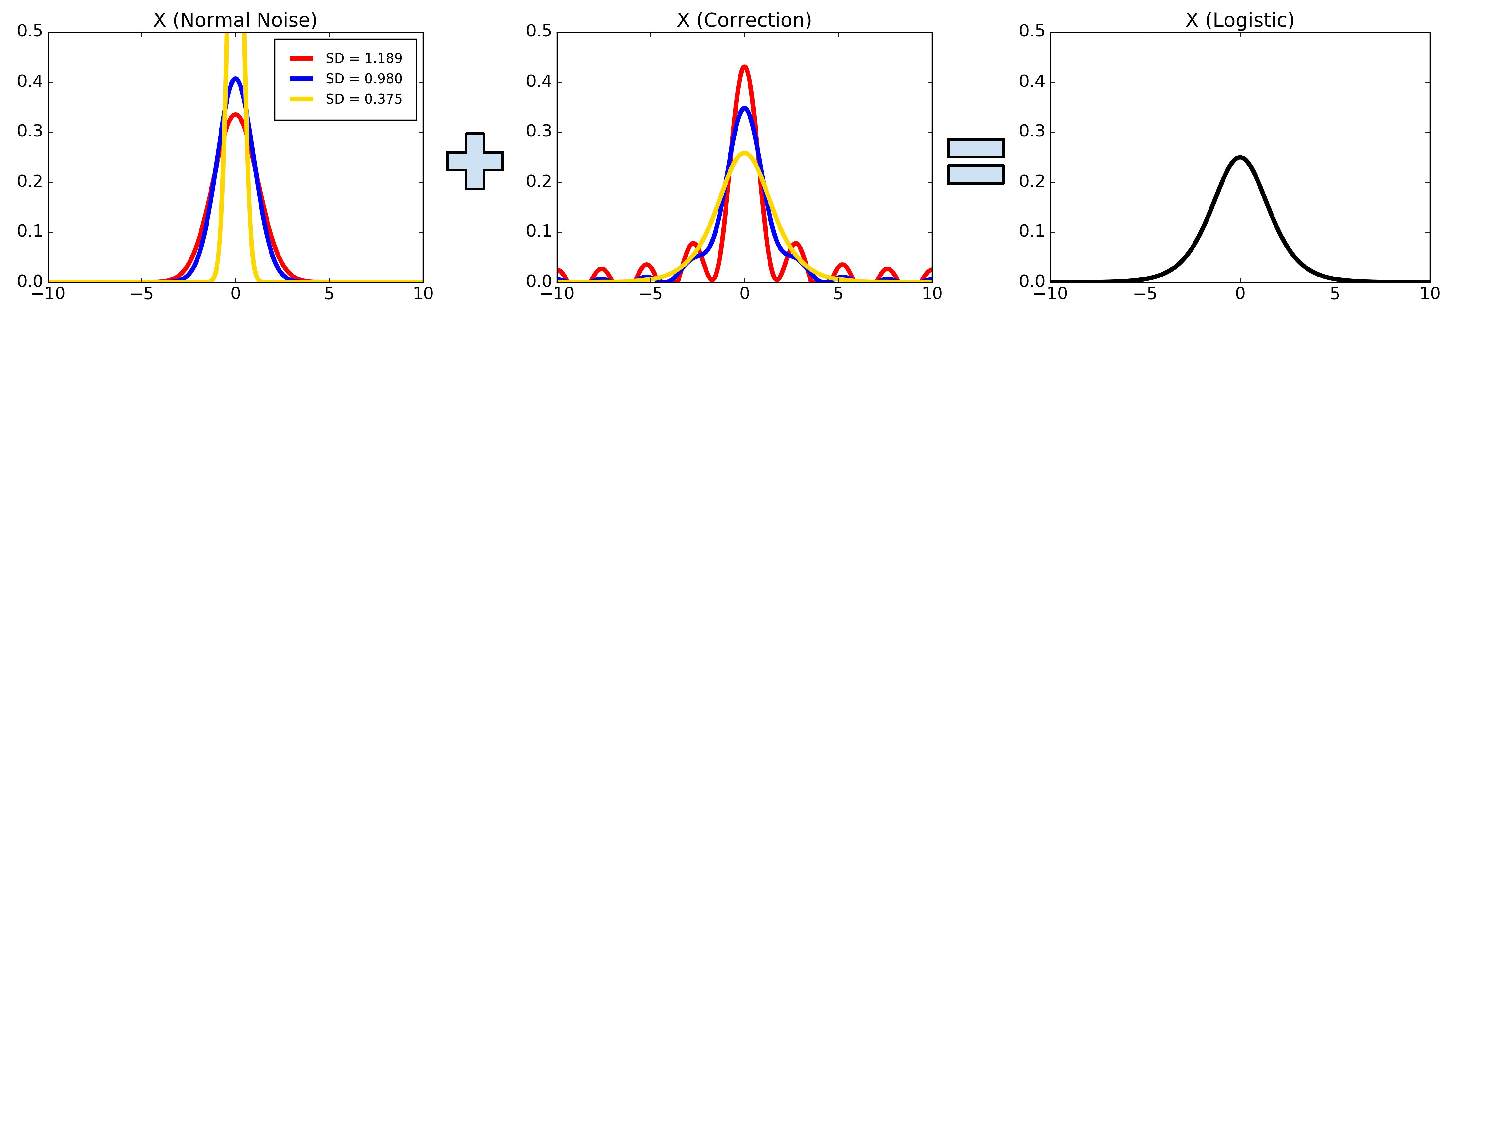
\includegraphics[width=1\textwidth]{mh_convolution_diagram_v2}
    \caption{
    Three examples of $X_{\rm norm}$ and $X_{\rm corr}$ distributions that
    convolve to form the standard logistic distribution. These were obtained
    based on our original linear programming formulation, as discussed in
    Section~\ref{sec:correction}. We use three standard deviation values of
    $X_{\rm norm}$. The two red curves convolve to form the logistic, etc. The
    $y$-axis is capped at 0.5 for readability. This figure must be viewed in
    color.
    }
    \label{fig:deconvolution}
    %\vspace{-10pt}
\end{figure}

Our proposed test in Equation~\ref{eq:criteria} requires knowing the
distribution of the correction variable $X_{\rm corr}$ such that $X_{\rm norm} +
X_{\rm corr} = X_{\rm log}$, where $X_{\rm norm} \sim \mathcal{N}(0,\sigma^2)$
and $X_{\rm log}$ has a standard logistic CDF, $(1+\exp(-X))^{-1}$. In
Section~\ref{sec:analysis}, we show that the accuracy of the test depends on the
absolute error between the CDFs of $X_{\rm norm} + X_{\rm corr}$ and $X_{\rm
log}$. Consequently, we need to minimize this in our construction of $X_{\rm
corr}$. More formally, let $\Phi_{s_X} = \Phi(X/s_X)$ where $\Phi$ is the
standard normal CDF\footnote{Hence, $\Phi_{s_X}$ is the CDF of a zero-mean
Gaussian with variance $s_X$.}, $S(X)$ be the logistic function, and
$C_{\sigma}(X)$ be the \emph{density} of the correction $X_{\rm corr}$
distribution. Our goal, based on Equation~\ref{eq:deconvolution}, is to solve
the following optimization problem:
\begin{equation}\label{eq:overall_corr_problem}
    C_\sigma^* = \argmin_{C_\sigma} |\Phi_{\sigma} * C_{\sigma} - S|
\end{equation}
where $*$ denotes convolution.

For computation of $C_\sigma$, we assume that its input $Y$ and
another variable $X$ lie in the intervals $[-V,V]$ and $[-2V,2V]$, respectively.
In continuous form, the optimization problem is therefore
\begin{equation}\label{eq:conv1}
    C_\sigma^* = \argmin_{C\sigma} \; \sup_{x \in [-2V,2V]}\left|\int_{-V}^{V}\Phi_{\sigma}(x-y) C_{\sigma}(y)dy - S(x)\right|
\end{equation}
To get $C_\sigma^*$ in a computable form, we discretize $X$ and $Y$ into $4N+1$
and $2N+1$ values respectively. If $i \in \{-2N, \ldots, 2N\}$ and $j \in \{-N,
\ldots, N\}$, then we can write $X_i = i(V/N)$ and $Y_j = j(V/N)$, and the
condition in Equation~\ref{eq:conv1} can be re-expressed as:
\begin{equation}\label{eq:conv2}
    C_\sigma^* = \argmin_{C_\sigma} \max_{i \in \{-2N,\ldots,2N\}}\left|\sum_{j = -N}^{N}\Phi_{\sigma}(X_i-Y_j) C_{\sigma}(Y_j) - S(X_i)\right|.
\end{equation}
To make the problem easier to understand, we can define a matrix $M$ and vectors
$u$ and $v$ such that $M_{ij} = \Phi_{\sigma}(X_i-Y_j)$, $u_j =
C_{\sigma}(Y_j)$, and $v_i = S(X_i)$, where the indices $i$ and $j$ are
appropriately translated to be non-negative indices for $M, u,$ and $v$. Thus,
Equation~\ref{eq:conv2} is equivalent to minimizing the $L_{\infty}$ norm:
\begin{equation}\label{eq:optimization_l1}
    u^* = \argmin_{u} \|Mu-v\|_{\infty}.
\end{equation}

We have the additional constraint that $u_j > 0$ for all $j$, since $u$
represents a density. We first explored optimizing this problem with linear
programming to find a $u$ minimizing $\|Mu - v\|_\infty$ subject to $u \ge 0$.
Figure~\ref{fig:deconvolution} shows three examples of $X_{\rm norm}$ and
$X_{\rm corr}$ densities that sum to $X_{\rm log}$ from this process.

This was tractable up to a few hundred dimensions for $u$.  However, the
discretization error is bounded by the curvature of the underlying functions
times the squared quantization step. The curvatures are here slightly less than
one, i.e.  the errors are of the order of $(V/N)^2$.  Here we chose $V=20$ to
provide adequate containment of the distributions (the CDFs are extremely close
to either zero or one outside this range). So with 200 points, we have a
discretization error of approximately 0.01, which is relatively large.  To yield
higher resolution and lower error, we switched to a least squares solution:
\begin{equation}\label{eq:optimization_l2}
    u^* = \argmin_u\; \|Mu-v\|_2^2 + \lambda \|u\|_2^2,
\end{equation}
where we add the standard regularization factor $\lambda$ for stability in high
dimensions. The solution is well-known from the normal equations: $u^* = (M^TM +
\lambda I)^{-1}M^Tv$, and in practice, it yields an acceptable $L_{\infty}$ norm for
Equation~\ref{eq:optimization_l1}.

With this approach, there is no guarantee that $u^* \geq 0$. However, we have
some flexibility in the choice of $\sigma$ in Equation~\ref{eq:conv1}.
As we decrease the variance of $X_{\rm norm}$, the variance of $X_{\rm corr}$
grows by the same amount and is in fact the result of convolution with a
Gaussian whose variance is the difference.  Thus as $\sigma$ decreases,
$C_\sigma(X)$ grows and approaches the derivative of a logistic function at
$\sigma = 0$. It retains some very weak negative values for $\sigma > 0$ but
removal of those values leads to very small error.

\SetKwInOut{Input}{Input}
\SetKwInOut{Output}{Output}
\begin{algorithm}[t]
\Input{Number of samples $T$, minibatch size $m$, error bound $\delta$, pre-computed correction $C_1(X)$ distribution, initial sample $\theta_1$.}
\Output{A chain of $T$ samples $\{\theta_1, \ldots, \theta_T\}$ from $p(\theta)$\;}
\For{$t=\{1, \ldots, T\}$}{
    Propose a candidate $\theta'$\ from proposal distribution $q(\theta'\mid\theta_t)$\;
    Draw a minibatch of $m$ points $x_i$, compute $\Delta^*(\theta_t,\theta')$ and sample variance $s^2_{\Delta^*}$\;
    Estimate moments $E|\Lambda_i-\Lambda|$ and $E|\Lambda_i-\Lambda|^3$ from the sample, and error $\epsilon$ from Equation~\ref{eq:clt-bounds3}\;
    \While {$s^2_{\Delta^*} \ge 1$ {\bf or} $\epsilon > \delta$}{
    	Draw $m$ more samples to augment the minibatch, update $\Delta^*$, $s^2_{\Delta^*}$ and $\epsilon$ estimates\;
    }
    Draw $X_{\rm nc} \sim \mathcal{N}(0,1-s^2_{\Delta^*})$ and
    $X_{\rm corr}$ from the correction distribution $C_1(X)$\;
        
        \eIf{$\Delta^* + X_{\rm nc} + X_{\rm corr} > 0$}{
            Accept the candidate, $\theta_{t+1} = \theta'$\;
        }{
            Reject and re-use the old sample, $\theta_{t+1} = \theta_t$\;
        }
    
}
\caption{A description of M-H sampling with our acceptance test.}
\label{alg:our_algorithm}
\end{algorithm}

\begin{table}[t]
    \caption{Error in $X_{\rm norm}+X_{\rm corr}$ versus $X_{\rm log}$}
    \label{tab:xcorr}
    \centering
    \begin{tabular}{l l l l}
    \toprule
    $N$ & $\sigma$ & $\lambda$ & $L_{\infty}$ error  \\
    \midrule
    4000 & 0.9 & 1 & 1.0e-4  \\
    4000 & 0.8 & 0.03 & 5.0e-6 \\
    \bottomrule
    \end{tabular}
\end{table}

As can be seen from Table~\ref{tab:xcorr}, the errors between $X_{\rm
norm}+X_{\rm corr}$ and $X_{\rm log}$ can be made very small, approaching single
floating precision (about $10^{-7}$). 

The complete procedure is given in Algorithm~\ref{alg:our_algorithm}. A few points:

\begin{itemize}
    \item It uses an adaptive step size so as to use the smallest possible
    average minibatch size. Unlike previous work however (and as we show in
    Section~\ref{sec:experiments}) the size distribution is short-tailed.

    \item An additional normal variable $X_{\rm nc}$ is added to $\Delta^*$ to
    produce a variable with unit variance. This is not mathematically necessary,
    but allows us to use a single correction distribution $C_1$ with $\sigma=1$
    for $X_{\rm corr}$, saving on memory footprint.

    \item The sample variance $s^2_{\Delta^*}$ is proportional to
    $\|\theta'-\theta\|_2^2$ whose distribution for Normal proposals is the
    square of a normal variable. 
\end{itemize}



\section{Analysis}\label{sec:analysis}

We now derive error bounds for our M-H test, and for the approximate target
distribution that it generates. From Table~\ref{tab:xcorr}, we know that
it is possible to generate the correction samples $X_{\rm corr}$ with a CDF
error approaching single-precision floating point error. We therefore treat the
$X_{\rm corr}$ variable as a sample from the exact correction distribution and
we will not analyze its errors.

In the most similar prior works,~\cite{cutting_mh_2014} uses asymptotic
arguments based on the Central Limit Theorem to argue that its approximate
acceptance test error tends to zero as batch size increases. But no quantitative
bounds are given. In~\cite{icml2014c1_bardenet14}, explicit bounds are given,
but they depend on bounding
\begin{equation}\label{eq:bad_bound}
    C_{\theta, \theta'} = \max_{1\leq i\leq N}|\log p(x_i\mid\theta') - \log p(x_i\mid\theta)|.
\end{equation}
Such bounds can be derived efficiently for models such as logistic regression,
but it is unclear how to derive them for a complex model such as a neural
network. In general, since a new $\theta'$ value is obtained each iteration, one
would need to iterate through all the $p(x_i\mid \theta')$ terms, defeating the
purpose of minibatch MCMC.

In this paper, we use quantitative forms of the Central Limit Theorem which rely
on measurable statistics from a single minibatch. Thus a sampler using our
approach does not need to ``see'' data beyond the current minibatch. This
supports use of the sampler on very large datasets, and in online mode where the
dataset is presented as a stream.

For the analysis, in Section~\ref{ssec:delta_star_distribution}, we first
present bounds on the absolute and relative error (in terms of the CDFs) of the
distribution of $\Delta^*$ vs a Gaussian. We then show in
Section~\ref{ssec:preserve_bounds} that these error bounds are preserved after
the addition of other random variables, in particular $X_{\rm nc}$ and $X_{\rm
corr}$. From this it follows that the acceptance test has the same error bound.

\subsection{Bounding the Distribution of $\Delta^*$ Versus a Gaussian}\label{ssec:delta_star_distribution}

To start, we use the following quantitative central-limit result:
  
\begin{lemma}\label{lem:quant_clt}
Let $X_1,\ldots,X_n$ be a set of zero-mean, independent, identically-distributed
random variables with sample mean $\bar{X}$ and sample variance $s^2_X$
where:
\begin{equation}
    \bar{X} = \frac{1}{n}\sum_{i=1}^nX_i \qquad {\rm and} \qquad s_X = \frac{1}{n}\left(\sum_{i=1}^n(X_i-\bar{X}^2\right)^{\frac{1}{2}}.
\end{equation}
This implies $t=\bar{X}/s_X$ has an approximate Student's distribution
which approaches a normal distribution in the limit. Then
\begin{equation}\label{eq:clt-bounds}
    \sup_x|{\rm Pr}(t<x) - \Phi(x)| \leq \frac{6.4E|X|^3+2E|X|}{\sqrt{n}}.
\end{equation}
\end{lemma}

\begin{proof}
The following bound is given immediately after Corollary 2 in from~\cite{explicit-clt05}:
\begin{equation}\label{eq:clt-boundsx}
-6.4E|X|^3-2E|X| \leq    \sup_x|{\rm Pr}(t<x) - \Phi(x)|{\sqrt{n}} \leq 1.36E|X|^3
\end{equation}
This bound applies to $x\geq 0$. Applying the bound to $-x$ when $x<0$
and combining with $x>0$, we obtain the weaker but unqualified bound
in Equation~\ref{eq:clt-bounds}.
\end{proof}

%% {\color{blue} Daniel: the notation here was (and still is, to a lesser extent)
%% the source of considerable confusion for me. Do we want $\sigma(X)$ or
%% $\sigma(\hat{X})$? I think in Lemma~\ref{lem:quant_clt} we want the former, not
%% the latter. OH ALSO, this section uses $n$ as the full data size, which means
%% before this section, we should use $n$, not $N$, for the full data size, right?
%% The Bardenet paper uses $n$ to represent the full data size.

%% JFC - this bound applies to minibatches, not the full dataset so the size $n$ is
%% deliberately not $N$.

Lemma~\ref{lem:quant_clt} demonstrates that as long as we know the first and
third absolute moments $E|X|$ and $E|X|^3$, we can bound the error of the normal
approximation, which decays as $O(n^{-\frac{1}{2}})$. Making the change of
variables $y = x s_X$, Equation~\ref{eq:clt-bounds} becomes
\begin{equation}\label{eq:clt-bounds2}
   \sup_y\left|{\rm Pr}(\bar{X}< y) - \Phi\left(\frac{y}{s_X}\right)\right| \leq \frac{6.4E|X|^3+2E|X|}{\sqrt{n}},
\end{equation}
showing that the distribution of $\bar{X}$ approaches the normal distribution
$\mathcal{N}(0,s_X)$ whose variance is $s_X$,
measured from the sample.

To apply this to our test, let $X_i = \Lambda_i(\theta,\theta') -
\Lambda(\theta,\theta')$, so that the $X_i$ are zero-mean, i.i.d. variables. If
instead of all $n$ samples, we only extract a subset of $b$ samples
corresponding to our minibatch, we can connect $\bar{X}$ with our $\Delta^*$
term:
\begin{equation}\label{eq:x-hat}
    \bar{X} = \Delta^*(\theta,\theta') - \Delta(\theta,\theta'),
\end{equation}
so that $s_X = s_{\Delta^*}$.
%{\color{blue} Daniel: This time it
%  makes sense to use $\sigma(\hat{X})$ instead of $\sigma(X)$.}
This results in the following Corollary:

\begin{corollary}\label{cor:our_bound_delta_prime}
We can now substitute into Equation~\ref{eq:clt-bounds2} and displace by the mean, giving:
\begin{equation}\label{eq:clt-bounds3}
    \sup_y\left|{\rm Pr}(\Delta^*< y) - \Phi\left(\frac{y-\Delta}{s_{\Delta^*}}\right)\right| \leq \frac{6.4E|X|^3+2E|X|}{\sqrt{b}} = \epsilon(\theta,\theta',b)
\end{equation}
\end{corollary}

Corollary~\ref{cor:our_bound_delta_prime} shows that the distribution of
$\Delta^*$ approximates a Normal distribution with mean $\Delta$ and variance
$s^2_{\Delta^*}$. Furthermore, it bounds the error with \emph{estimable
quantities}: both $E|X|$ and $E|X|^3$ can be estimated as means of $|\Lambda_i
- \Lambda|$ and $|\Lambda_i - \Lambda|^3$, respectively, on each minibatch. We
expect this will often be accurate enough on minibatches with hundreds or
thousands of points, but otherwise bootstrap CIs can be computed from those
sequences. Since the bounds are monotone in $E|X|$ and $E|X|^3$, using upper
bootstrap CI limits will provide high-confidence error bounds.



\subsection{Bounds are Preserved After Adding Random Variables}\label{ssec:preserve_bounds}

We next relate the CDFs of distributions and show that bounds are preserved
after adding random variables.

\begin{lemma}\label{lem:cdf_bounds}
Let $P(x)$ and $Q(x)$ be two cumulative distributions satisfying
$\sup_x|P(x)-Q(x)|\leq \epsilon$ with $x$ in some real range. Let $R(y)$ be the
{\em density} of another random variable $y$. Let $P'$ be the convolution $P*R$
and $Q'$ be the convolution $Q*R$. Then $P'(z)$ (resp. $Q'(z)$) is the CDF of
sum $z=x+y$ of independent random variables $x$ with CDF $P(x)$ (resp. $Q(x)$)
and y with density $R(y)$.  Then
\begin{equation}
    \sup_x|P'(x)-Q'(x)|\leq \epsilon
\end{equation}
\end{lemma}

\begin{proof}
We first observe that
\begin{equation}\label{eq:pdf_difference}
    P'(z) - Q'(z) = \int_{-\infty}^{+\infty}(P(z-x)-Q(z-x))R(x) dx,
\end{equation}
and since $\sup_x|P(x)-Q(x)|\leq \epsilon$ it follows that for all $z$:
\begin{equation}
-\epsilon = \int_{-\infty}^{+\infty} -\epsilon R(x) dx \leq \int_{-\infty}^{+\infty}(P(z-x)-Q(z-x))R(x) dx \leq \int_{-\infty}^{+\infty}\epsilon R(x) dx = \epsilon
\end{equation}
\end{proof}

%% {\color{blue} Daniel: Hold on, the following Corollary seems to add $X_{\rm norm}$
%% to both random variables we are comparing (and \emph{then} $X_{\rm corr}$). But
%% didn't the previous section already justify that $\Delta^* \approx \Delta +
%% X_{\rm norm}$? That is, I don't think we need to add another $X_{\rm norm}$; I
%% think we just want to add $X_{\rm corr}$. Otherwise, this new test does not
%% match what we wrote earlier.

%% I think the easiest way to resolve this is to do the following: we assume that
%% $\Delta^*$ is already $\Delta + X_{\rm noise}$. Then all we need to do is add
%% $X_{\rm corr}$. So this is the same as what we are doing, except we do not need
%% to apply Lemma~\ref{lem:cdf_bounds} twice; we just need to do it once because we
%% are only adding $X_{\rm corr}$, not $X_{\rm norm}$.}

Relating Lemma~\ref{lem:cdf_bounds} to our acceptance test, we observe that:

\begin{corollary}\label{cor:bounds_preserved}
If $\sup_y|{\rm Pr}(\Delta^* < y) - \Phi(\frac{y-\Delta}{s_{\Delta^*}})|
\leq \epsilon(\theta,\theta',b)$, then
\begin{equation}
    \sup_y|{\rm Pr}(\Delta^*+X_{\rm nc}+X_{\rm corr} < y) - S(y-\Delta)| \leq \epsilon(\theta,\theta',b)
\end{equation}
where $S(x)$ is the standard logistic function, and $X_{\rm nc}$ and $X_{\rm corr}$ are generated as per Algorithm 1. 
\end{corollary}

\begin{proof}
We apply Lemma~\ref{lem:cdf_bounds} twice. First take:
\begin{equation}
    P(y) = {\rm Pr}(\Delta^* < y) \qquad {\rm and}\qquad Q(y) = \Phi\left(\frac{y-\Delta}{s_{\Delta^*}}\right)
\end{equation}
and convolve with the distribution of $X_n$ which has density $\phi(X/\sigma_n)$
where $\sigma_n^2 = 1 - s^2_{\Delta^*}$. This yields the next iteration of $P$
and $Q$:
\begin{equation}
    P'(y) = {\rm Pr}(\Delta^*+X_{\rm nc} < y) \qquad {\rm and}\qquad Q'(y) = \Phi\left({y-\Delta}\right)
\end{equation}
Now we convolve with the distribution of $X_{\rm corr}$ which gives:
\begin{equation}
    P''(y) = {\rm Pr}(\Delta^*+X_{\rm nc}+X_{\rm corr} < y) \qquad {\rm and}\qquad Q''(y) = S\left({y-\Delta}\right)
\end{equation}
Both steps preserve the error bound $\epsilon(\theta,\theta',b)$. Finally
$S(y-\Delta)$ is a logistic CDF centered at $\Delta$, and so $S(y-\Delta) = {\rm
Pr}(\Delta + X_{\rm log} < y)$ for a logistic random $X_{\rm log}$. We conclude
that the probability of acceptance for the actual test ${\rm Pr}(\Delta^*+X_{\rm
nc}+X_{\rm corr} > 0)$ differs from the exact test ${\rm Pr}(\Delta+X_{\rm
log} > 0)$ by at most $\epsilon$.
\end{proof}

As our discussion in Section~\ref{sec:our_algorithm} showed, as the distribution
of $\Delta^*$ approaches a Gaussian, our new MH test becomes more accurate.
Corollary~\ref{cor:bounds_preserved} shows that the bounds from
Section~\ref{ssec:delta_star_distribution} are preserved after the addition of
the random variables we use, showing that our test should remain accurate.

%% {\color{blue} Daniel: Do we want to include this new analysis? There seem to be
%% two different ways we show the bound. The first part (above) is nice and I like
%% it (and it seems to show all we need for Algorithm 1, doesn't it?}

In fact we can do better than this approximation (showing the error decreases as
$O(n^{-1})$) by using a more precise limit distribution under an additional
assumption. Let $\mu_i$ denote the $i^{th}$ moment, and $b_i$ denote the
$i^{th}$ absolute moment of $X$. If Cramer's condition holds:
\begin{equation}\label{eq:cramers_condition}
    \lim_{t \to \infty} \sup |E(\exp(i t X))| < 1,
\end{equation}
then Equation 2.2 in Bentkus et al.'s work on Edgeworth
expansions~\cite{Bentkus97} provides the following:

\begin{lemma}\label{lem:clt_edgeworth}
Let $X_1,\ldots,X_n$ be a set of zero-mean, independent, identically-distributed
random variables with sample mean $\hat{X}$ and with $t$ defined as in Lemma 3.
If $X$ satisfies Cramer's condition, then
\begin{equation}\label{eq:clt-bounds_edgeworth}
    \sup_x\left|{\rm Pr}(t<x) - G\left(x, \frac{\mu_3}{b_2^{3/2}}\right)\right| \leq \frac{c(\epsilon,b_2,b_3,b_4,b_{4+\epsilon})}{n}
\end{equation}
where
\begin{equation}
    G_n(x,y) = \Phi(x) + \frac{y(2x^2+1)}{6\sqrt{n}}\Phi'(x).
\end{equation}
\end{lemma}

Lemma~\ref{lem:clt_edgeworth} shows that the average of the $X_i$ has a more
precise, skewed CDF limit $G_n(x,y)$ where the skew term has weight proportional
to a certain measure of skew derived from the moments:
$\frac{\mu_3}{b_2^{3/2}}$. Note that if the $X_i$ are symmetric, the weight of
the correction term is zero, and the CDF of the average of the $X_i$ converges
to $\Phi(x)$ at a rate of $O(n^{-1})$.

Here the limit $G_n(x,y)$ is a normal CDF plus a correction term that decays as
$n^{1/2}$.
%{\color{blue} (Daniel: how did the equation in the next sentence
% appear? I verified it and it seems correct, but it looks like it popped out of
%nowhere.)}
% JFC: It comes from taking a second derivative. You dont need to explain it. 
Importantly, since $\phi^{''}(x) = x^2\phi(x) - \phi(x)$ where
$\phi(x)=\Phi'(x)$, the correction term can be rewritten giving:
\begin{equation}\label{eq:GNderivatives}
    G_n(x,y) = \Phi(x) + \frac{y}{6\sqrt{n}}(2\phi^{''}(x)+3\phi(x))
\end{equation}
From which we see that $G_n(x,y)$ is a linear combination of $\Phi(x)$,
$\phi(x)$ and $\phi^{''}(x)$. This is quite fortuitous. In Algorithm 1, we
correct for the difference in $\sigma$ between $\Delta^*$ and the variance
needed by $X_{\rm corr}$ using $X_{\rm nc}$. This same method works when we
wish to estimate the error in $\Delta^*$ vs $G_n(x,y)$. Since all of the
component functions of $G_n(x,y)$ are derivatives of a (unit variance)
$\Phi(x)$, adding a normal variable with variance $\sigma'$ increases the
variance of all three functions to $1+\sigma'$. Thus we add $X_{\rm nc}$ as
per Algorithm 1 preserving the limit in Equation~\ref{eq:GNderivatives}.

The deconvolution approach can be used to construct a correction variable
$X_{\rm corr}$ between $G_n(x,y)$ and $S(x)$ the standard logistic function. An
additional complexity is that $G_n(x,y)$ has additional parameters $y$ and $n$.
Since these act as a single multiplier $\frac{y}{6\sqrt{n}}$ in
Equation~\ref{eq:GNderivatives}, its enough to consider a function $g(x,y')$
parametrized by $y'= \frac{y}{6\sqrt{n}}$. This function can be computed and
saved offline. As we have shown above, errors in the ``limit'' function
propagate directly through as errors in the acceptance test.  To achieve a test
error of $10^{-6}$ (close to single floating point precision), we need a $y'$
spacing of $10^{-6}$. It should not be necessary to tabulate values all the way to
$y'=1$, since $y'$ is scaled inversely by the square root of minibatch size.
Assuming a max $y'$ of 0.1 requires us to tabulate about 100,000.  Since our $x$
resolution is 10,000, this leads to a table with about 1 billion values, which
can comfortably be stored in memory.  However, if $g(x,y)$ is moderately smooth
in $y$, it should be possible to achieve similar accuracy with a much smaller
table. We leave further analysis and experiments with $g(x,y)$ as future work.
%{\color{blue} Daniel: I will look at the code to understand this paragraph
%better because right now I am confused.}
% JFC: the code doesnt implement this yet.




\section{Experiments}\label{sec:experiments}

We conduct two sets of experiments to explore the benefits of our minibatch MH
test and to benchmark it with previous work. In Section~\ref{ssec:gaussians}, we
show that our test enables samples to converge to the posterior distribution of
a heated Gaussian mixture model. In Section~\ref{ssec:logistic}, we analyze its
efficiency on logistic regression.  Appendices~\ref{app:gaussian}
and~\ref{app:logistic} contain more detailed information on these respective
experiments.

\subsection{Mixture of Gaussians}\label{ssec:gaussians}

We start with a simple Gaussian mixture model, borrowing an experiment
from~\cite{langevin_2011}.  The parameter is 2-D, $\theta =
\langle \theta_1,\theta_2 \rangle$, and the parameter/data generation process is
%% \begin{equation}\label{eq:data_generation}
%%     (\theta_1,\theta_2) \sim \mathcal{N}((0,0), {\rm diag}(\sigma_1^2, \sigma_2^2));\quad \quad x_i \sim
%%     0.5 \cdot \mathcal{N}(\theta_1, \sigma_x^2) + 0.5 \cdot \mathcal{N}(\theta_1+\theta_2, \sigma_x^2).
%% \end{equation}
\begin{equation}\label{eq:data_generation}
    \begin{bmatrix} \theta_1 \\ \theta_2 \end{bmatrix} 
    \sim \mathcal{N}\left(\begin{bmatrix}0 \\ 0\end{bmatrix}, 
    \begin{bmatrix} \sigma_1^2 & 0 \\ 0 & \sigma_2^2\end{bmatrix} \right);\quad \quad x_i \sim
    0.5 \cdot \mathcal{N}(\theta_1, \sigma_x^2) + 0.5 \cdot \mathcal{N}(\theta_1+\theta_2, \sigma_x^2).
\end{equation}
We set $\sigma_1^2 = 10, \sigma_2^2 = 1$ and $\sigma_x^2=2$.  We fix $\theta =
\langle 0,1 \rangle$. The original paper sampled 100 data points from this
distribution, and estimated the posterior in the parameters. We are interested
in performance on larger problems and so sampled 1,000,000 points to form the
posterior of $p(\theta)\prod_{i=1}^{1,000,000}p(x_i\mid \theta)$ with the same
prior from Equation~\ref{eq:data_generation}. The larger number of samples
produces a much sharper posterior with two very narrow peaks.  Our goal is to
reproduce the original posterior, so we adjust the temperature to $T=10,000$.
Taking logs, we get the target as shown in the far left of
Figure~\ref{fig:gauss_mix_1}.

We run MCMC with our MH test using minibatch size $m=100$.  We also run this
using the methods from~\cite{cutting_mh_2014} (``Korattikara 2014'')
and~\cite{icml2014c1_bardenet14} (``Bardenet 2014''), also with $m=100$.
For~\cite{cutting_mh_2014}, we increment minibatches by 100 as recommended, and
for~\cite{icml2014c1_bardenet14}, we increase the minibatch size geometrically
with a ratio of $\gamma = 1.5$ as recommended. These tests use different
minibatch size updates because of their different approaches to repeated
testing. \cite{icml2014c1_bardenet14} uses straightforward discounting,
allocating a fraction of the test error $\delta$ to each minibatch test (call
these subtests). Its important to bound the number of subtests therefore, so
that the tolerable error per subtest is not too small.  \cite{cutting_mh_2014}
uses a more aggressive repeated testing approach, explicitly modeling
correlation between tests and allowing many more tests for a given $\delta$. 

The tolerance for making a decision in~\cite{cutting_mh_2014} is
$\epsilon=0.005$, and the error bound control parameters
in~\cite{icml2014c1_bardenet14} are $p = 2$ and $\delta = 0.01$.  All methods
(including ours) use the same random walk proposer with covariance $\Sigma={\rm
diag}(0.3, 0.3)$.  Since the proposer generates a random walk, all shaping of
distribution of the samples is due to the MH test. All methods are run 5000
times to collect 5000 samples.

\begin{figure}[t]
    \centering
    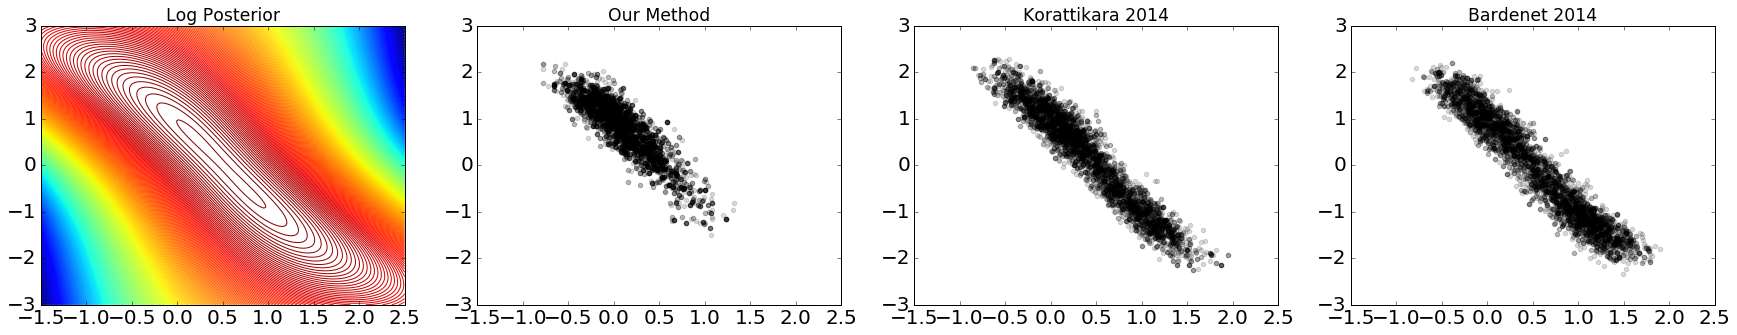
\includegraphics[width=1\linewidth]{GaussianMixtureResult/posterior_of_gaussian.png}
    \caption{
    The log posterior contours and scatter plots of sampled $\theta$ values
    using different methods. 
    }
    \label{fig:gauss_mix_1}
\end{figure}

\begin{figure}[t]
    \centering
    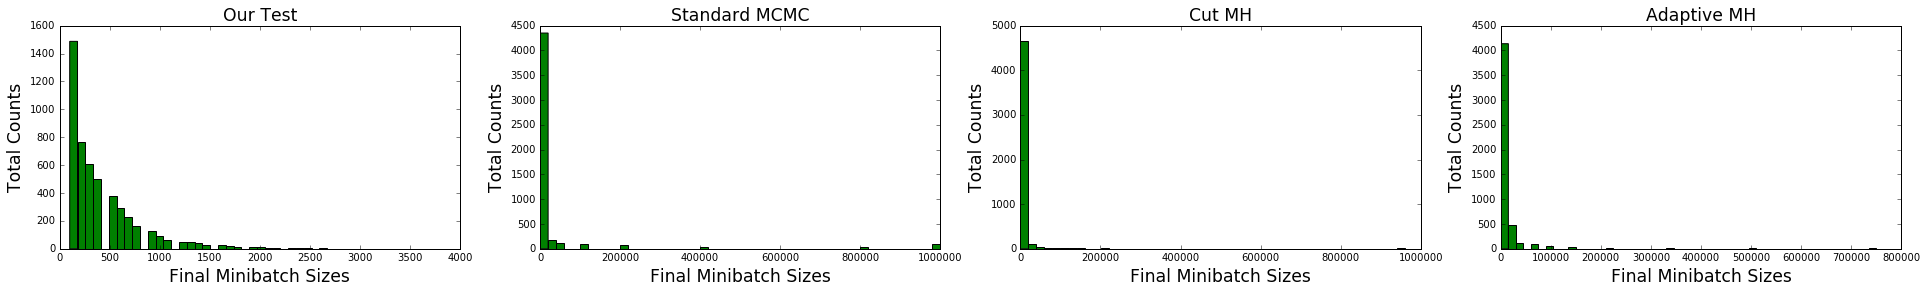
\includegraphics[width=1\linewidth]{minibatch_size_gaussian.png}
    \caption{
    Counts of minibatch sizes that the three methods used in the experiment of
    Section~\ref{ssec:gaussians}. To make comparisons easier, the axes have the
    same range (using a log-log scale).
    }
    \label{fig:gauss_mix_2}
\end{figure}

Figure~\ref{fig:gauss_mix_1} shows scatter plots of the resulting $\theta$
samples for the three methods, with darker regions indicating a greater density
of points. There are no obvious differences, so to better understand any
differences, we measure the similarity between each set of samples and the
actual posterior. 

To effect the comparison, we first discretize the posterior coordinates into
bins (non-overlapping ranges) with respect to the two components of the
parameter $\theta$.  The probability of a sample falling into one of these bins
is the integral of the true posterior probability over the area of that bin. Let
this probability be denoted $P_i$ where $i$ is the bin number. A single sample
from any of the MH methods should therefore be multinomial with distribution
$P$, and a set of $n$ (ideally independent) samples should follow a ${\rm
Multinomial}(P,n)$ distribution.  Since the ideal distribution is simple, we can
use it to measure the quality of the sample distributions rather than use
general purpose tests like KL-divergence or likelihood-ratio.  The latter in any
case are problematic with zero counts in some bins as we have here.

In practice, it is difficult to compute multinomial probabilities for large $n$,
in that case the per-bin distributions are well-approximated by Poisson
distributions with parameter $\lambda_i=P_i n$. Given a set of samples $\Theta =
\{\theta_1,\ldots,\theta_T\}$, let $c_j$ denote the number of individual samples
$\theta_i$ that fall in bin $j$. Then the log probability for the set is
approximated as
\begin{equation}\label{eq:log_prob_poissons}
    \log p(\Theta) \approx \frac{1}{N_{\rm bins}} \sum_{j=1}^{N_{\rm bins}} c_j \log (n P_j) - n P_j - \log(\Gamma(c_j+1)).
\end{equation}
The results for each model are shown in Table~\ref{tab:poissons} ...
{\color{blue} Daniel: IN PROGRESS}

While the Poisson results provide general guidance on the relative accuracy of
the models it is difficult interpret the quantitative scores. We therefore
perform significance tests to test the null hypothesis that the ideal
distribution really generated the samples.  We perform two tests:

\begin{enumerate}
    \item An exact test using simulation to generate an approximate distribution
    of scores given the null hypothesis.

    \item An approximate test using the chi-squared distribution as the test
    statistic. 
\end{enumerate}

The results were... {\color{blue} Daniel: IN PROGRESS}

Figure~\ref{fig:gauss_mix_2} shows a histogram of the final minibatch sizes used
by the three methods in each iteration. Our method consumes significantly less
data; most minibatch sizes are smaller than 1000, and the average size is 210.
The other methods occasionally need to consume a large proportion of the
entire data set of one million elements; the average minibatch sizes are 14862
and 18098 for Korattikara 2014 and Bardenet 2014, respectively. The average
minibatch sizes accurately predict the running times of these methods since
all methods have a running time proportional to the total data consumed, with
one caveat: the method of~\cite{icml2014c1_bardenet14} requires a global bound
on the term $C_{\theta,\theta'}$ (see Equation~\ref{eq:bad_bound}) over the
entire the data set at every iteration in order to calculate the error bound.
This bound must be either computed analytically using properties of the specific
dataset, or it must be checked at each sample if a black-box test is required.
We found that the sample code provided by the authors
of~\cite{icml2014c1_bardenet14} in fact computed this bound explicitly for each
sample generated, i.e. the implementation traversed the entire dataset for each
sample, providing no performance advantage over the complete test. For this
reason, we omitted the time to compute $C_{\theta,\theta'}$ from our
measurements of the running time of the sample implementation
of~\cite{icml2014c1_bardenet14}, and consider only the time to process the
minibatches.

%% In Figure ~\ref{fig:gauss_bardenet}, the value
%% of the first part and second part of equation (9)
%% in~\cite{icml2014c1_bardenet14} is shown with respect to the size of actual
%% minibatch data used. The second part which contains  the $C_{\theta,\theta'}$
%% term is larger than the first part, which means that the second part is
%% non-negligible and has to be calculated at every iteration. This is one of the
%% very time-consuming parts in this method.  {\color{blue} Daniel: I am not sure
%% if we should include this plot. Let me think about it and if we decide to
%% include it I will help rewrite the explanation.}

%% JFC - it would still be interesting to see this comparison, however:
%% (i) its important to include equation (9) and explain what the terms are.
%% (ii) the results dont look right. I wouldnt expect the first term to be
%% so small compared to the second and I'm fairly certain they should cross
%% in the illustrated range. It would be better to include both curves on
%% the same plot. 

\begin{table}[t]
    \caption{\color{blue} Daniel: TODO Poisson Probabilities}
    \label{tab:poissons}
    \centering
    \begin{tabular}{l l l l}
    \toprule
    Model & Ours & Korattikara 2014 & Bardenet 2014 \\
    \midrule
    Poisson Value (Eq.~\ref{eq:log_prob_poissons}) & TODO & TODO & TODO \\
    \bottomrule
    \end{tabular}
\end{table}




\subsection{Logistic Regression}\label{ssec:logistic}

We next use logistic regression for the binary classification of 1s versus 7s in
the MNIST dataset~\cite{lecun-mnisthandwrittendigit-2010}. The data has 12007
training and 1000 testing elements (we used a random subset of the test data).
For the proposer, we use a random walk with covariance matrix $0.05I$ for the
$784\times 784$ identity matrix $I$. We set the posterior temperature at
$T=1000$ and use the minibatch size $m=100$ and compare
with~\cite{cutting_mh_2014} with tolerance 0.005 and
with~\cite{icml2014c1_bardenet14} with error bound control parameters $p = 2$
and $\delta = 0.01$.
% {\color{blue} Daniel: just observed this, but why are we
% using a subset of the test data? We really should use all 2000 (I think it's
% 2000, right?).}
% JFC- Would be good to fix, but not critical.

Figure~\ref{fig:logistic_performance} shows the prediction accuracy and log
likelihood on the test set as a function of the cumulative training data points
processed.  We see that our minibatch MH test is more efficient compared to the
other two methods, because it has similar or better performance while consuming
fewer data points.

\begin{figure}[t]
	\centering
	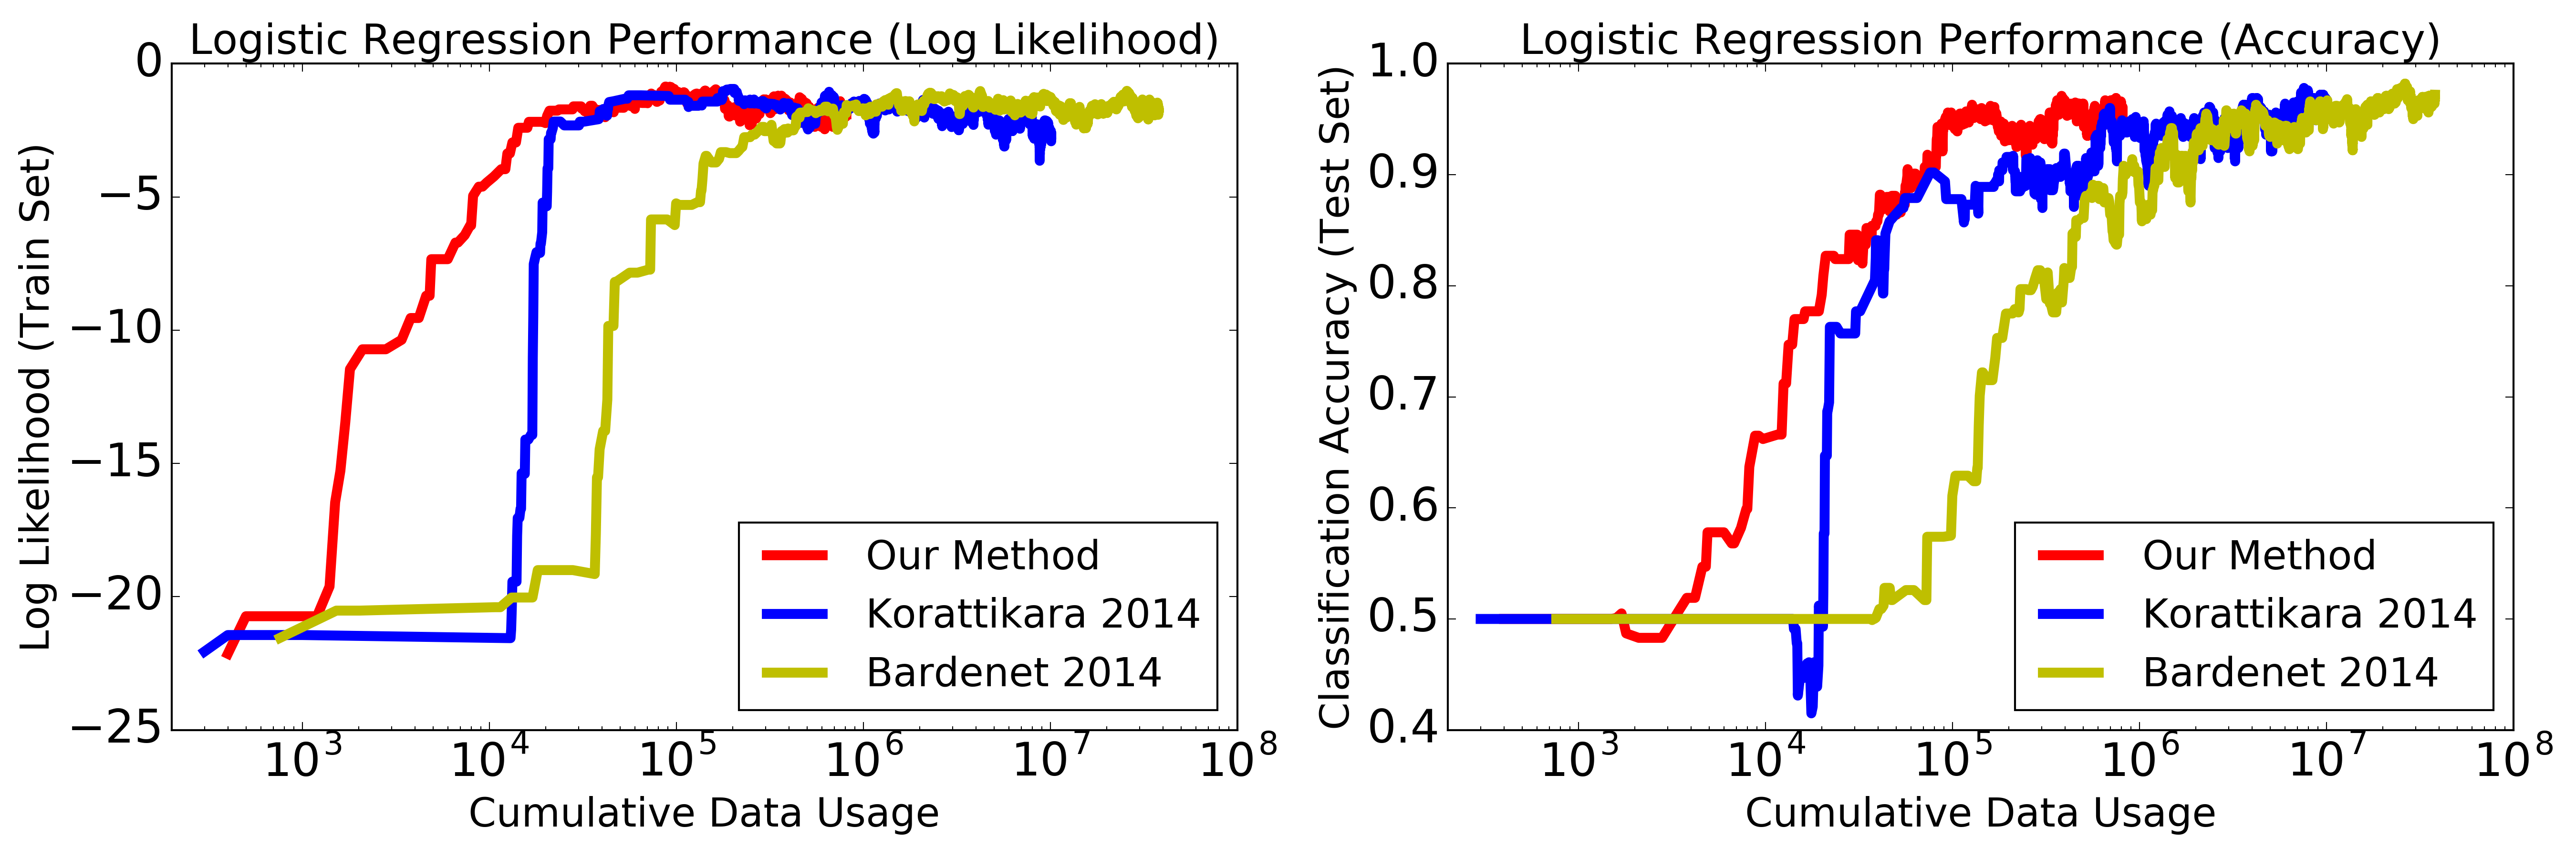
\includegraphics[width=1\linewidth]{logistic_performance.png}
	\caption{
    Logistic regression performance (accuracy/log likelihood) based on
    cumulative data usage.
    }
	\label{fig:logistic_performance}
\end{figure}


\begin{figure}[t]
	\centering
	\includegraphics[width=1\linewidth]{minibatch_size_logistic.png}
	\caption{
    Counts of minibatch sizes that the three methods used in the MNIST logistic
    regression experiment from Section~\ref{ssec:logistic}. It is analogous to
    Figure~\ref{fig:gauss_mix_2}.
    }
	\label{fig:logistic_minibatch}
\end{figure}

Figure~\ref{fig:logistic_minibatch} shows the histogram of minibatch sizes for
all three methods. With an initial minibatch size of 100, Korattikara 2014 and
Bardenet 2014 achieve average minibatch size of 2026 and 7612 respectively over
the MNIST classification task, while our method achieves that of 163, showing
significantly better performance than the benchmark test methods.



\section{Conclusions}\label{sec:conclusion}

In this paper, we have derived a new MH test for minibatch MCMC methods. We
demonstrated how a simple deconvolution process allows us to use a minibatch
approximation to the full data tests. We experimentally show the benefits of our
test on Gaussian mixtures and logistic regression.  Straightforward directions
for future work include running more experiments with a particular focus on
investigation of the variance precondition.  More elaborate extensions include
testing on deep neural networks and combining our results with Hamiltonian Monte
Carlo methods, providing a recipe for how to use our algorithm (following the
framework of~\cite{sgmcmc_2015}), or integrating parallel
MCMC~\cite{conf/uai/AngelinoKWSA14,conf/icml/AhnSW14} concepts.


\small
\bibliography{nips_2016}
\bibliographystyle{ieeetr}
\normalsize

\clearpage
\appendix

\begin{center}
{\Large Outline of Appendix}
\end{center}

In this appendix, we describe the following topics:

\begin{itemize}[noitemsep]
    \item The proof of Lemma~\ref{lem:worst_case}.
    \item More information on Section~\ref{ssec:gaussians}.
    \item More information on Section~\ref{ssec:logistic}.
\end{itemize}

\section{Proof of Lemma~\ref{lem:worst_case}}\label{app:worst_case_proof}

Assume $(\theta' - \theta) \in \pm\frac{1}{\sqrt{N}}[0.5,1]$ and $\theta -0.5
\in \pm\frac{1}{\sqrt{N}}[0.5,1]$ with matching sign. These events occur with
probability ({\color{blue} Daniel: sorry for interjecting here but don't we need
to take into account the $1/\sqrt{N}$ in the probabilities? If $N \to \infty$
(and it's going to be large with big datasets) the probabilities should be about
zero.}) $p_0=2*(\Phi(1)-\Phi(0.5)) = 0.2997$ and
$p_1=(\Phi(1)-\Phi(0.5))=0.14988$ respectively, and guarantee that
$\Lambda^*(\theta',\theta)$ is negative. This then guarantees that we can find a
$u \in [0,1]$ so that $\psi(u,\theta',\theta)$ equals
$\mathbb{E}[\Lambda^*(\theta',\theta)]$.  Specifically, choose $u_0$ to satisfy
\begin{equation}\label{eq:log_uo}
    \log u_0 = N(\Lambda^*(\theta',\theta)-\psi(1,\theta',\theta))
\end{equation}
which evaluates ({\color{blue} Daniel: sorry again for interjecting but I really
think $\log u_0$ does not have that $N$ there. Also, for the subsequent
equation, I think we need to be using \emph{expected} values of $\Lambda^*$}) to
\begin{equation}
    \log u_0 = -N(\theta'-\theta)\left(\theta-0.5+\frac{\theta'-\theta}{2}\right).
\end{equation}
This means we can rewrite the acceptance test as
\begin{equation}
    \frac{1}{b}\sum_{i=1}^b x_i-\left(\theta+\frac{\theta'-\theta}{2} + \frac{\log u_0}{N(\theta'-\theta)}\right)
    \hspace{0.1in} \not\approx \hspace{0.1in} 0
\end{equation}
where $\not\approx$ means ``significantly different from'' under the
distribution over samples of $x_i$.  The above choice of $u_0$ ensures that the
terms in parenthesis above sum to 0.5. Since the $x_i$ have mean 0.5, the test
will never correctly succeed.  Furthermore, if we sample values of $u$ near
enough to $u_0$, the terms in parenthesis will not be sufficiently different
from 0.5 to allow the test to succeed. 
  
{\color{blue} Daniel: I would like to ask you about these probabilities because
I do not know how we got these intervals.} The choices above for $\theta$ and
$\theta'$ guarantee that
\begin{equation}
    \log u_0 \in -[0.5,1][0.75,1.5] = -[0.375,1.5]
\end{equation}
and consider the range of $u$ values
\begin{equation}
    \log u \in \log u_0 + [-0.5,0.375]
\end{equation}
the size of the range in $u$ is at least $\exp([-2,-1.125]) = [0.13534,0.32465]$ and occurs
with probability at least $p_2=0.18932$. With $u$ in this range, we rewrite the test as:
\begin{equation}
    \frac{1}{b}\sum_{i=1}^b x_i-0.5 \hspace{0.1in} \not\approx \hspace{0.1in} \frac{\log u/u_0}{N(\theta'-\theta)}
\end{equation}
so that the LHS has expected value zero.  Given our choice of intervals for the
variables, the RHS is in the range $1/\sqrt{N}[-1,0.75]$.  The standard
deviation of the LHS given the interval constraints is at least $0.5/\sqrt{b}$.
And so the gap between LHS and RHS is at most $2\sqrt{b/N}$ standard deviations. 

The samples $\theta$, $(\theta'-\theta)$ and $u$ are drawn independently and so
the probability of the conjunction of these events is $c = p_0 p_1 p_2 =
0.0085$.



\section{Gaussian Mixture Experiment Details}\label{app:gaussian}

In this section, we provide more details on Section~\ref{ssec:gaussians}.  Our
parameter is a 2-D vector
$\theta = \langle \theta_1, \theta_2 \rangle$, where
\begin{equation}
\theta_1 \sim \mathcal{N}(0, \sigma_1^2) \quad \mbox{ and } \quad \theta_2 \sim \mathcal{N}(0, \sigma_2^2)
\end{equation}
and where $\mathcal{N}$ indicates the normal distribution (more generally, the
multivariate normal). We consider the above as our prior.
Following~\cite{langevin_2011}, we set $\sigma_1^2 = 10$ and $\sigma_2^2=1$, so
the covariance matrix of $\theta$ is $\Sigma = {\rm diag}(10,1)$. Therefore, the
log prior probability we endow on $\theta$ is
\begin{equation}
\log p(\theta) = \log \left(\frac{1}{2\pi\sqrt{10}}\right) - \frac{1}{2}\theta^T\Sigma^{-1}\theta.
\end{equation}
To generate the data, we use the following Gaussian mixture with tied means:
\begin{equation}\label{eq:x_points}
x_i \sim \frac{1}{2}\mathcal{N}(\theta_1, \sigma_x^2) + \frac{1}{2}\mathcal{N}(\theta_1+\theta_2, \sigma_x^2)
\end{equation}
where, again following~\cite{langevin_2011}, we set $\sigma_x^2 = 2$. This means
the log likelihood of a single data instance is
\begin{equation}
\log p(x_i \mid \theta) = \log \frac{1}{4\sqrt{\pi}} +
\log\left(\exp\left(-\frac{1}{4}(x_i - \theta_1)^2\right) + \exp\left(-\frac{1}{4}(x_i -
(\theta_1+\theta_2))^2\right)\right)
\end{equation}
The official problem statement is as follows: given some number of conditionally
independent data points $x_1, x_2, \ldots, x_N$ generated according
to~(\ref{eq:x_points}), determine the posterior distribution of $\theta$:
\begin{equation}\label{eq:log_post}
\log p(\theta \mid x_1,\ldots,x_N) = \log p(\theta) + \sum_{i=1}^N\log p(x_i \mid \theta).
\end{equation}
Alternatively, depending on the application, we may opt to instead pick a point
estimate\footnote{We do this for the logistic regression experiment, described
in Section~\ref{ssec:logistic} and elaborated in Appendix~\ref{app:logistic}.}
of $\theta$, such as the MAP estimate. (If $N$ is extremely large, it will cause
the posterior to peak sharply at its modes, reducing distribution estimates to
point estimates.)

One technique we use to make our test more applicable is to add a temperature to
the posterior. In general, we will add $T > 1$ so that the posterior is
$p(\theta)(\prod_{i=1}^N p(x_i\mid \theta))^{1/T}$, resulting in the log
posterior of 
\begin{equation}\label{eq:log_prior_temp}
\log p(\theta \mid x_1,\ldots,x_N) \approx \log p(\theta) + \frac{1}{T}\sum_{i=1}^N\log p(x_i \mid \theta).
\end{equation}
which has the extra $1/T$ to decrease the scale factor, so the variance scales
as $1/T^2$.

% Daniel: I decided that I don't like this figure anymore.
% \begin{figure}[t]
%   \centering
%   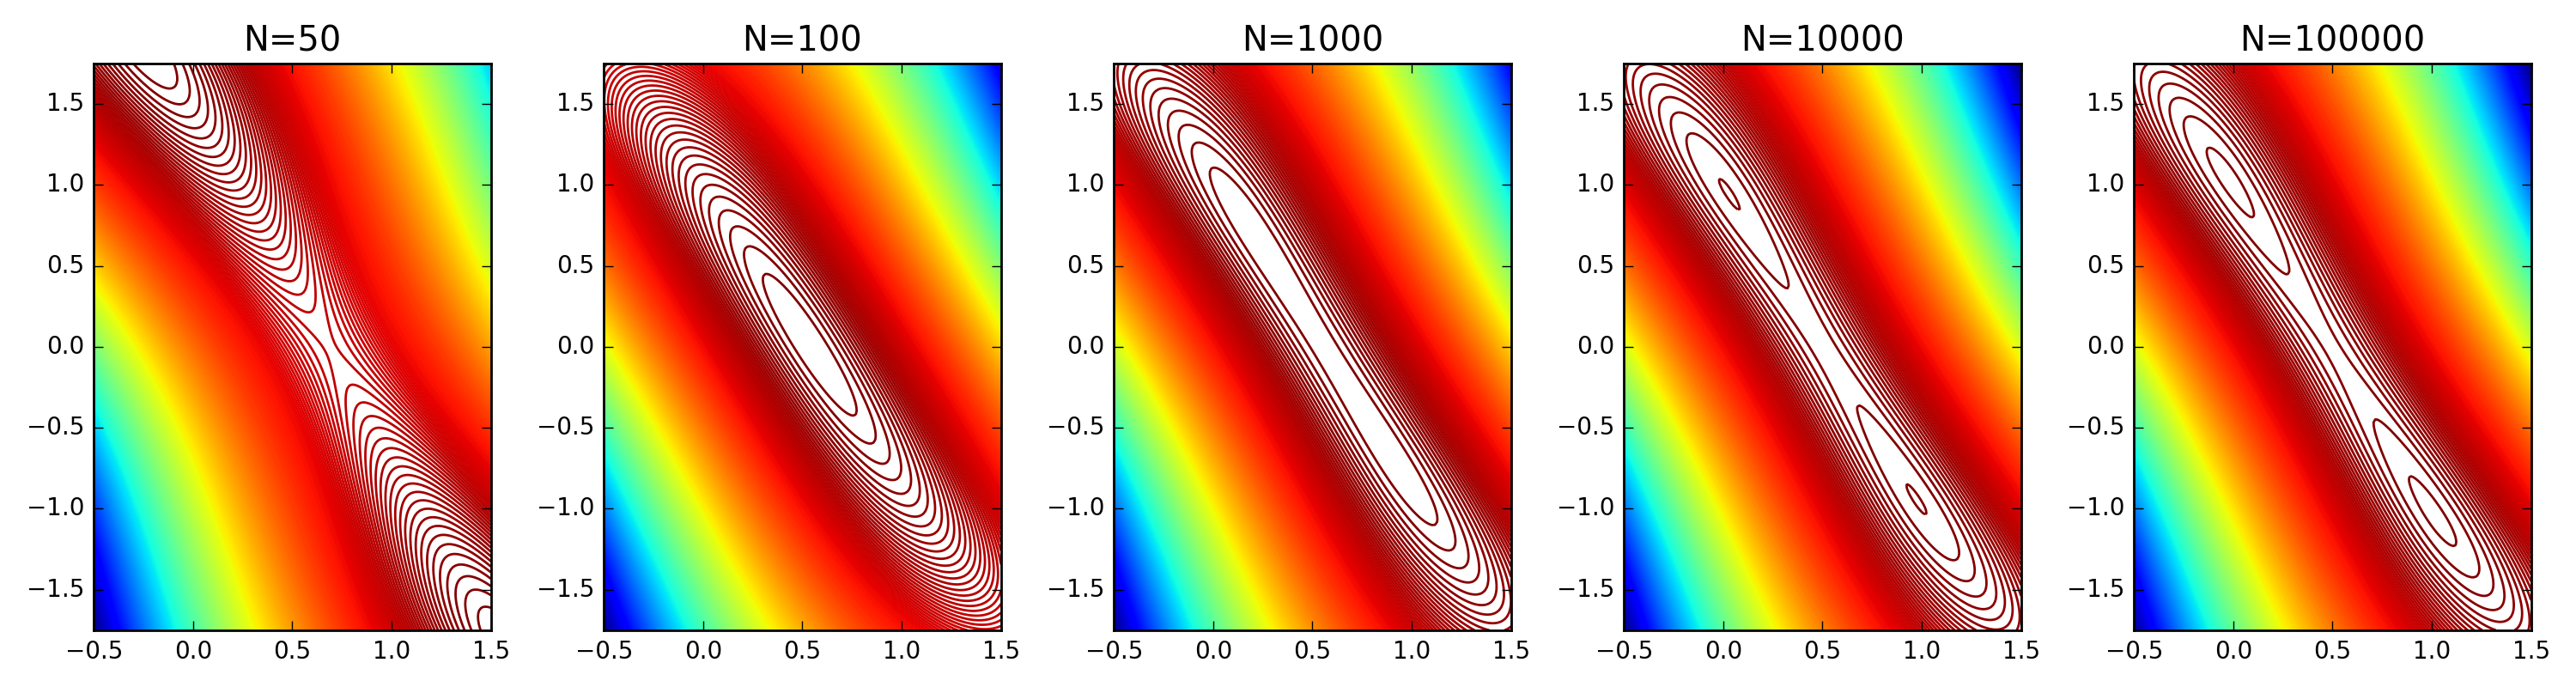
\includegraphics[width=1\linewidth]{contour_v1}
%   \caption{The posterior distribution, from 50 to 100k samples, with temperature set at 1.}
%   \label{fig:contour1}
% \end{figure}

\begin{figure}[t]
  \centering
  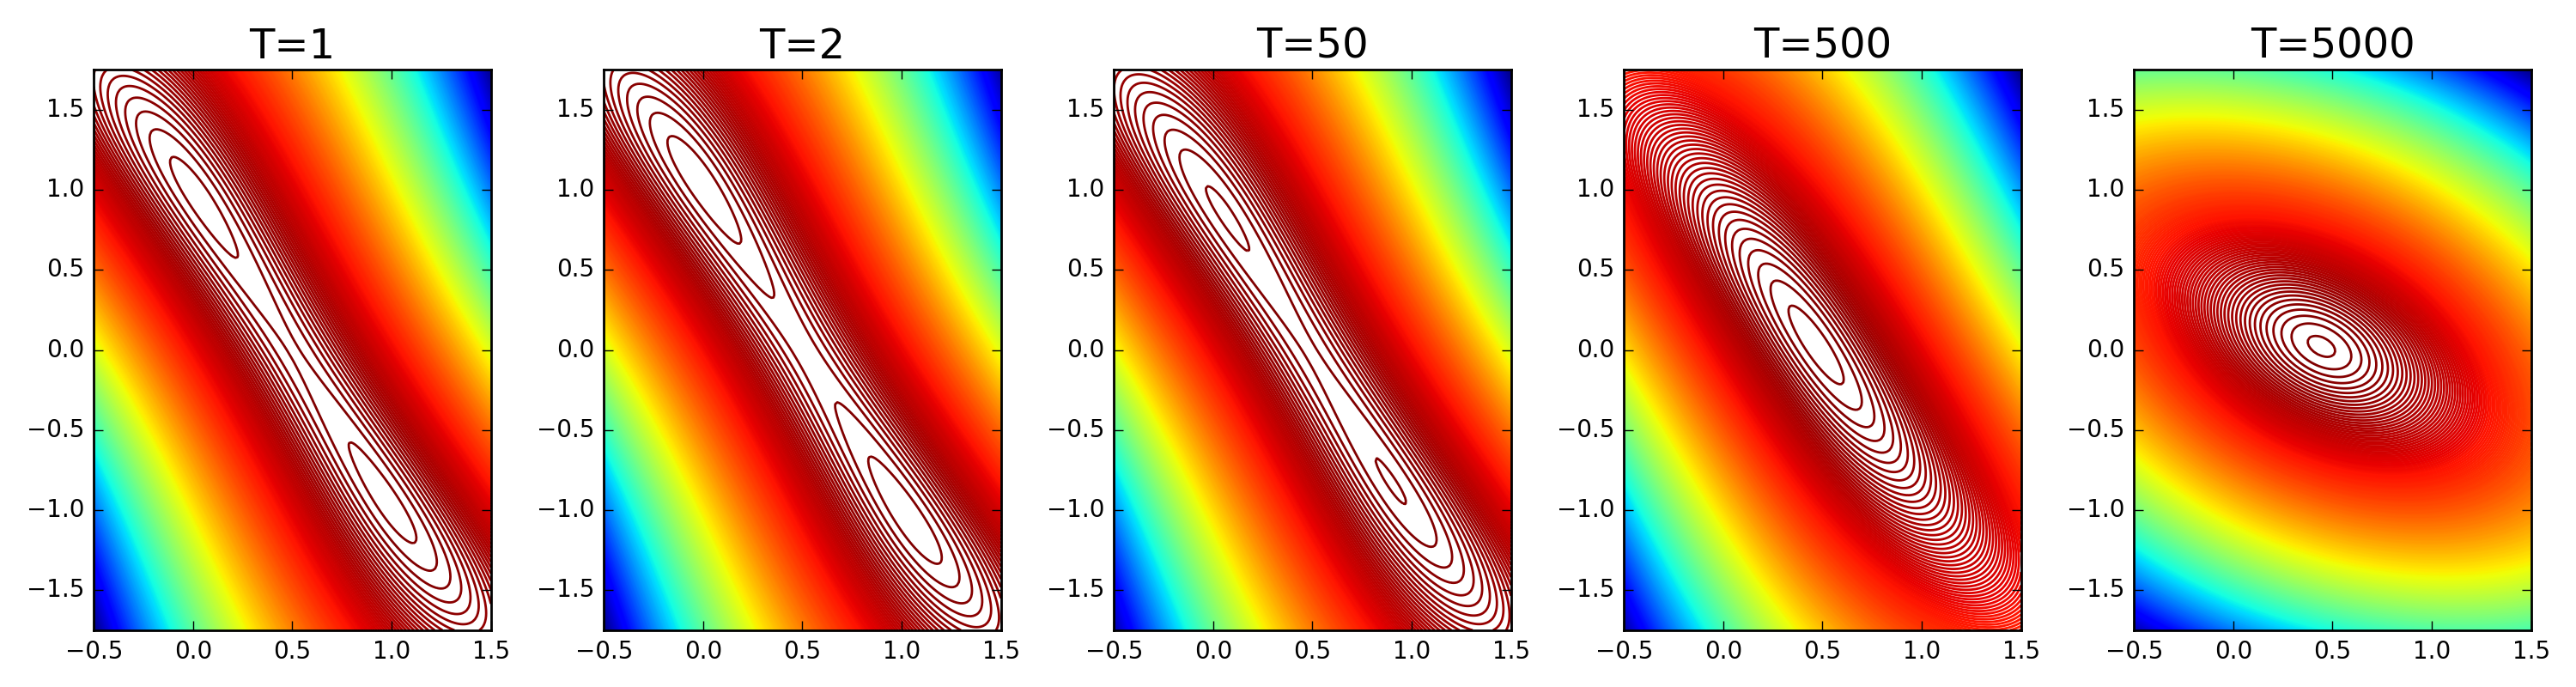
\includegraphics[width=1\linewidth]{contour_v2}
  \caption{The posterior distribution, with $N=10000$ and temperature $T$ varying.}
  \label{fig:contour2}
\end{figure}

To gain intuition on the shape of the posterior, Figure~\ref{fig:contour2} shows
simulated contour plots of the posterior based on $N=10000$ data points, and
temperature varying.  The (non-tempered) posterior is a multimodal distribution
with modes at $(0,1)$ and $(1,-1)$. A larger $T$ implies a flatter posterior,
which can be useful for parameter exploration so that the samples do not get
trapped in a mode.


\section{Logistic Regression Experiment Details}\label{app:logistic}

In this section, we go over some details of our logistic regression experiment. The feature vector
for an image consists of its pixel values, normalized between 0 and 1. For simplicity, we only
consider the binary classification case, so we only use digits one (denoted as output $y = 1$) and
seven (denoted as $y = -1$). The probability of the $i^{\rm th}$ output $y_i \in \{-1,+1\}$ with the
input vector $x_i$ is
\begin{equation}
p(y_i \mid x_i) = \frac{1}{1+\exp (-y_i \theta^T x_i)},
\end{equation}
where $\theta$ is the 784-length parameter vector.

For our experiment, we impose a uniform prior to represent our lack of knowledge about $\theta$.  We
use a random walk proposer, which can be modeled as $\theta' = \theta_i + \mathcal{N}(0,
\sigma^2I)$, where $\theta_i$ is the current sample, $\theta'$ is the proposed sample, and we choose
the variance to be a constant $\sigma^2 = 0.05$ for all components. We initialize $\theta_0$ to be a
vector of all ones, and set our minibatch size as $m=100$.

For our minibatch MH test, in order to enforce the ${\rm std}(\Delta') < 1.2$ condition, we use a
constant temperature $T = 1000$. If our estimated ${\rm std}(\Delta') \ge 1.2$, we ignore the
current iteration.  %Figure~\ref{fig:appendixExp2} plots our estimated ${\rm std}(\Delta')$ values
%versus iteration count. 

%\begin{figure}[t]
  %\centering
  %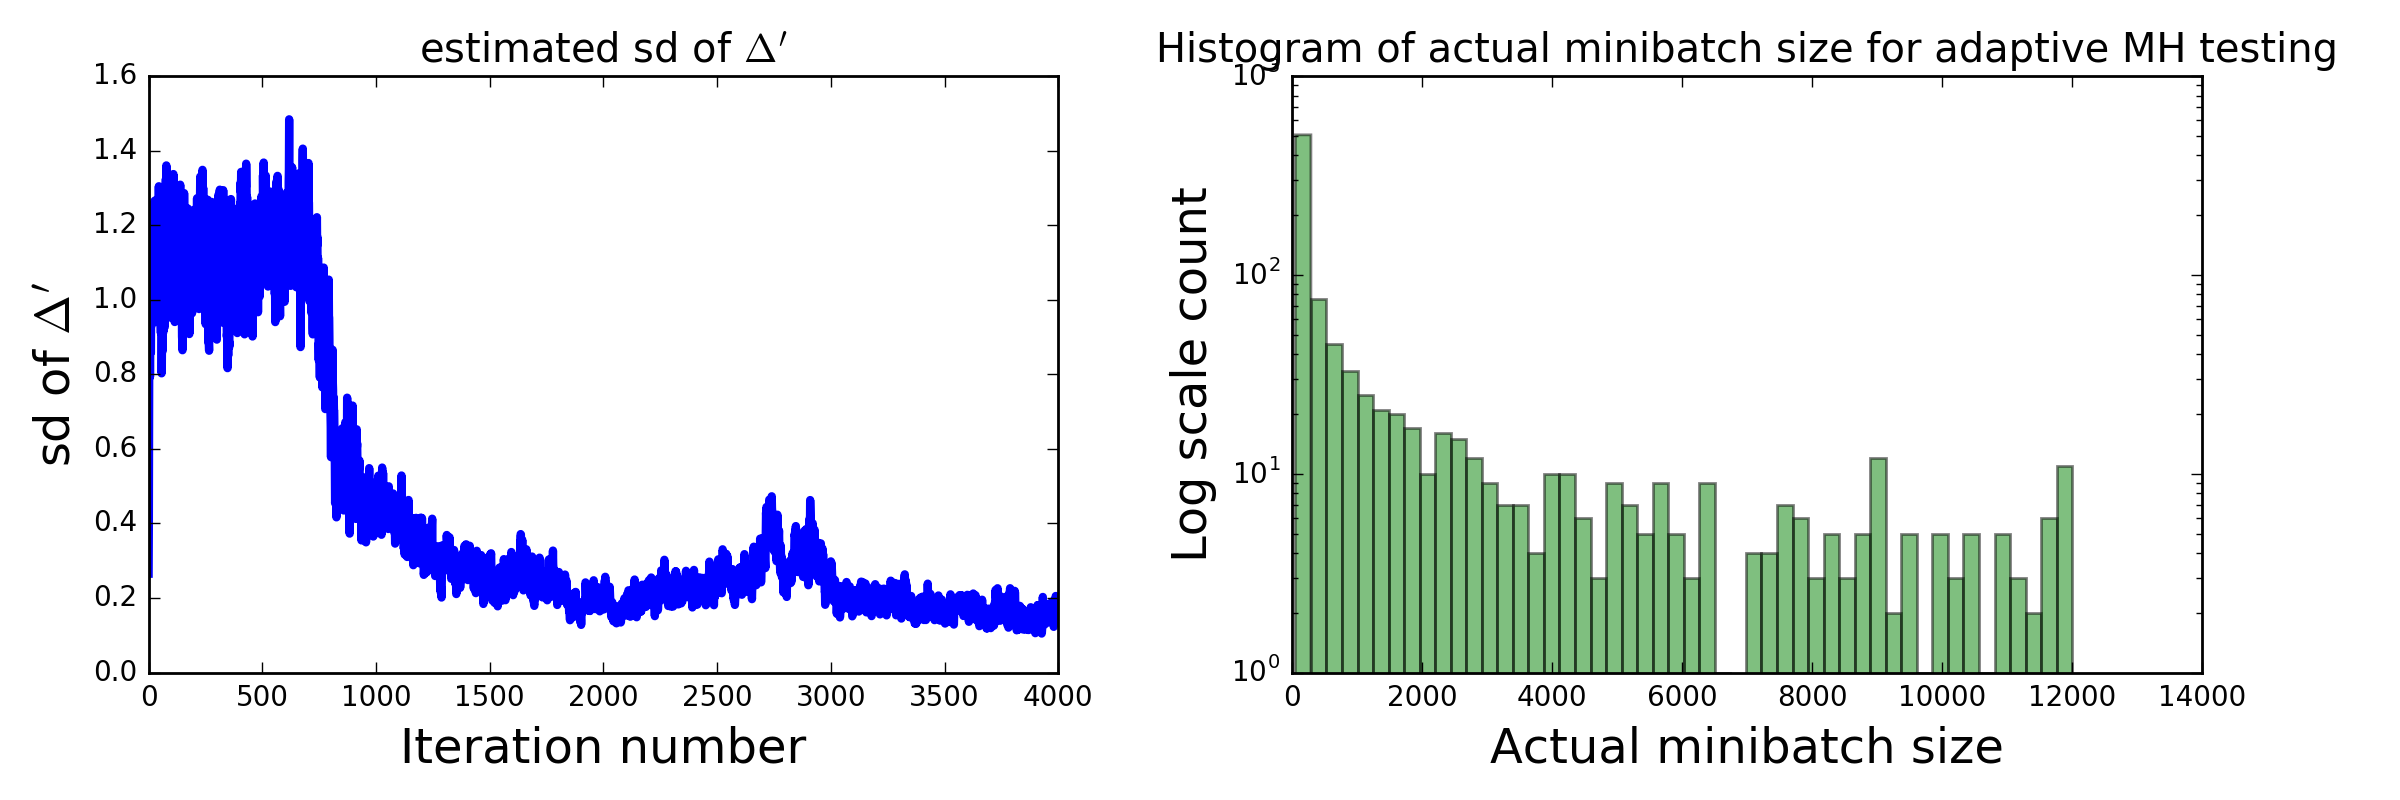
\includegraphics[width=1\linewidth]{./figures/appendixExp2}
 % \caption{Additional results for the logistic regression experiment.}
  %\label{fig:appendixExp2}
%\end{figure}

%For adaptive MH testing, our experimental settings are the same as with our MH test, except we do
%not impose a temperature. The minibatch size of adaptive MH testing is also initialized as 50, but
%it may increase by that amount each iteration. Figure~\ref{fig:appendixExp2} shows the histogram of
%the actual minibatch size at the end of each iteration in adaptive MH testing.

\iffalse
\section{Neural Network Experiment Details}\label{app:nnet}

For our neural network experiment, we use the architecture discussed in Section~\ref{ssec:nets}. We
use the SGHMC as the proposer for our minibatch MH testing. For the baseline, we use a tuned
adaptive gradient descent optimizer, whose step size changes by $0.01 /(i+1)^{0.4}$. Both methods
have minibatch sizes set at $m=200$. There are one million total data instances $x_i$.

For SGHMC, we use the simplified update equations~\cite{sghmc_2014}:
\begin{equation}
\Delta \theta = v, \quad \quad\Delta v = -\eta \nabla U(\theta) - \alpha v + \mathcal{N}(0, 2(\alpha
-\hat{\beta}) \eta),
\end{equation}
where $v$ represents auxiliary momentum variables, and $\nabla U(\theta)$ is the gradient of the
system. We set the hyperparameters to be $\eta_i = 0.01 /(i+1)^{0.4}$, and $\alpha=0.1$. We use the
empirical Fisher~\cite{conf/icml/AhnBW12} information $V(\theta)$ to estimate the value of
$\hat{\beta}$, so that $\hat{\beta}=\frac{1}{2}\eta V(\theta)$. In order to control ${\rm
std}(\Delta')$, we initialize the temperature at 1000, and adjust it at iteration $i$ according to
$T_i = \max\{1, 1000/(i+1)^{0.5}\}$.

\fi



% Daniel: here are example LaTeX codes for figures and tables if we want to use them.
%\begin{figure}[h]
%  \centering
%  \fbox{\rule[-.5cm]{0cm}{4cm} \rule[-.5cm]{4cm}{0cm}}
%  \caption{Sample figure caption.}
%\end{figure}
%\begin{table}[t]
%  \caption{Sample table title}
%  \label{sample-table}
%  \centering
%  \begin{tabular}{lll}
%    \toprule
%    \multicolumn{2}{c}{Part}                   \\
%    \cmidrule{1-2}
%    Name     & Description     & Size ($\mu$m) \\
%    \midrule
%    Dendrite & Input terminal  & $\sim$100     \\
%    Axon     & Output terminal & $\sim$10      \\
%    Soma     & Cell body       & up to $10^6$  \\
%    \bottomrule
%  \end{tabular}
%\end{table}
%\usepackage[pdftex]{graphicx} ...
%\includegraphics[width=0.8\linewidth]{myfile.pdf}

\end{document}

